% $Id$

Chapter \ref{ch:findchirp} described the algorithms that we use to generate
inspiral triggers given an inspiral template and a \emph{single data segment}.  There
is more to searching for gravitational waves from binary inspiral than trigger
generation, however. To perform a search for a given class of sources in a
large quantity of interferometer data we construct a \emph{detection
pipeline}.  In section \ref{s:construction} we give an overview of the
the components used in a pipeline and how they fit together.
We then describe the building blocks of the pipeline in more detail. Section
\ref{s:dq} describes data quality cuts, which are used to discard 
data which is unsuitable for analysis. The application of trigger generation
to the data is explained in section \ref{s:pipetemplate}. The use of data from
multiple interferometers is described in section \ref{s:coincidence}. In
section \ref{s:vetoes} we show how data from the interferometer that does not
measure the gravitational wave signal can be used.  Finally in section
\ref{s:s2pipeline} we describe the pipeline that has been constructed to
search for binary neutron stars and binary black hole MACHOs in the S2 data.

\section{Construction of Inspiral Pipelines}
\label{s:construction}

A detection pipeline is a sequence of operations that starts with the raw data
from the interferometers and produces a list of \emph{candidate events}.
Figure \ref{f:simple_pipe} shows a simple pipeline to filter the data from a
pair of interferometers labeled IFO$1$ and IFO$2$.
We only use data that comes from interferometers in stable operation. Running
an interferometer is a complex process that requires human \emph{operators}
who are trained to \emph{lock} the interferometers. Locking the interferometer
is the process of bringing it from an uncontrolled state 
to a state where light is resonant in the interferometer.  From a
state in which the interferometer optics are freely swinging, the operators
manually align the optics of the interferometer using the interferometer
control systems. They then direct the automated lock acquisition
system\cite{Evans:thesis} to bring the Fabry-Perot cavities into resonance
with the beam splitter positioned so that the light at the anti-symmetric
port is a minimum. The recycling cavity is then brought into resonance and the
length sensing and control servo maintains the locked state by monitoring the
motion of the optics and adjusting their position accordingly.   In addition
to the operator, members of the LIGO Scientific Collaboration trained in the
operation of the interferometer are present at the observatory. The
collaboration member on duty is known as the as scientific monitor or
\emph{scimon}. Once the interferometer is locked, the operator and scimon
decide if the quality of the data being recorded is suitable to be flagged as
\emph{science mode data}. If the data is suitable it passes the first cut for
gravitational wave analysis and the operators and scimons continuously monitor
the data using various \emph{data monitoring tools}. Lock is lost
when the length sensing servo no longer has enough dynamic range to maintain
resonance in the interferometer. This is typically caused by large seismic
events which may be local to the observatory (e.g. liquid nitrogen tanks
creaking as the expand in the sun) or of global origin (e.g. a large
earthquake in China has caused loss of lock). Poor data quality in the
interferometer may also require a break in lock to remedy.  Continuous
locked operation has been maintained for up to $66.2$~hours in
the Hanford 4km interferometer. Seismic noise in the Livingston interferometer
limited the longest lock to $6.93$~hours during S2.

It is possible that the operators or scimons may make mistakes in deciding
that data should be flagged as science mode; they may forget to enable
calibration lines, for example. There may also be noise sources or transient
events in the data which make it unsuitable for analysis but which are not
easily detectable in the control room while the data is being taken. To
prevent such data from being used in an astrophysical analysis a list of
\emph{data quality cuts} is compiled. The manual selection of science mode
data may be considered the first data quality cut.  Additional tests of data
quality are described in section \ref{s:dq}.

The chirp signals from compact binary inspiral depend on the masses and spins
of the binary elements, as described in section \ref{s:inspiralgw}. Searching
for gravitational waves from BBHMACHOs requires signals which only depend on
the masses $m_1$ and $m_2$ of the binary.  The inspiral signals from BBHMACHOs
lie in some region of the template parameter space described by the component
masses $m_1$ and $m_2$. A single template is not sufficient to search for
signals from the population, as the template for a given pair of mass
parameters may not produce a high signal-to-noise ratio when used as a filter
to detect a signal with different mass parameters.  To search for signals from
a \emph{region} of parameter space we construct a \emph{bank} of inspiral
templates as described in section \ref{s:pipetemplate}. The template bank is
constructed to cover the parameter space in such a way that we do not discard
any signals from our target population.

We then use the bank of templates to filter the data for inspiral signals using
the matched filter and $\chi^2$ veto discussed in chapter \ref{ch:findchirp}.
This results in a list of \emph{inspiral triggers}. For the pipeline shown in
figure \ref{f:simple_pipe}, a bank of templates is generated used to filter
the data for inspiral signals for each interferometer. We describe how trigger
generation is used in a pipeline in section in detail in section
\ref{s:pipetemplate}.

One of the most powerful methods of rejecting false alarms is coincidence
between different interferometers. As described previously, there are three
LIGO interferometers which are operated simultaneously during science runs.
The H1 and H2 detectors are co-located at the LIGO Hanford Observatory and the
L1 detector is located at the LIGO Livingston Observatory. A true
gravitational wave should produce a signal in all operating detectors at the
same time, up to the time delay for the arrival of the wavefront of the
gravitational wave at the observatories.  We therefore require \emph{time
coincidence}, which demands that inspiral triggers be present in all operating
detectors simultaneously, with time offsets less than the light travel time
between detectors plus the measurement error of detection. While coincidence
is the most obvious use of multiple interferometers, other coincidence tests
may also be used, e.g. demanding consistency of the waveform parameters
between the triggers from two detectors, or consistency in the recovered
amplitude of the signal relative to the sensitivity of the detectors. We
describe these tests in section \ref{s:coincidence}.

While the goal during data acquisition is to ensure that the data recorded is
as stationary and Gaussian as possible, transient noise artifacts may still be
present in the data. For example, it has been seen that a person jumping up
and down in the control room at the observatory will cause a burst of noise in
the gravitational wave channel. There may also be occasional glitches in the
interferometer control systems that cause a transient in the gravitational
wave channel, despite the best efforts of the experimental team. To allow us
to distinguish such events from true gravitational wave signals, we record
several thousand data streams of auxiliary interferometer control channels and
physical environment monitor (PEM) channels. Auxiliary channels monitor the
state of the servo loops that control the interferometer and include
information about the pre-stabilized laser, the length sensing and control
system and the input and output optics.  PEM channels record the data from
devices such as seismometers, magnetometers and microphones placed in and
around the interferometer. These devices are designed to detect environmental
sources that may couple to signals in the gravitational wave channel. This
data can be used to construct \emph{vetoes} of the inspiral triggers if a
coupling can be identified between a noise source present in an auxiliary or
PEM channel and inspiral triggers in the gravitational wave channel.  We
demonstrate this process with examples in section \ref{s:vetoes}. 

The final step in constructing a pipeline is to turn the various elements
described above (data quality cuts, template bank generation, trigger
generation, coincidence and vetoing) into code that can be executed in an
automated way on a computing cluster. The execution of the code must ensure
that all the input data has been analyzed and the components of the pipeline
are executed in the correct sequence. We use a directed acyclic graph
(DAG) to describe the work flow of a pipeline.  For example, we may
construct construct a DAG to execute the simple pipeline in figure
\ref{f:simple_pipe} on all the data from L1 and H1 recorded in S2. The DAG
describing the work flow is submitted to a computing cluster via the Condor
high throughput computing system\cite{beowulfbook-condor}. The Condor DAG
manager executes the pipeline described in the DAG that we generate. This
process is described in more detail in section \ref{ss:dag}.

Implicit in the above discussion is that fact that there are many parameters
that must be set at each stage of the pipeline. For example: What data quality
cuts should we use? What signal-to-noise and $\chi^2$ thresholds should we use
when generating the inspiral triggers? What coincidence tests should we apply
and what should their parameters be? What auxiliary channels and PEM channels
should be used as vetoes, and how do we apply these vetoes to inspiral
triggers? Answering these questions is the key to turning a pipeline into a
full binary inspiral search; we call the process of selecting the parameters
\emph{tuning the pipeline}. In fact, pipeline tuning and construction of the
pipeline are not entirely separate. After constructing a pipeline and initial
tuning, we may decide to revisit the pipeline topology before performing
additional tuning.

When tuning the pipeline we may wish to minimize the \emph{false alarm rate},
i.e. minimize the number of candidate events that are not due to inspiral
signals.  We may simultaneously wish to minimize the false dismissal rate to
ensure that the pipeline does not discard triggers that are due to real
signals.  The false alarm rate can be studied by looking at candidate events
in the playground. The false dismissal rate can be studied by \emph{injecting}
signals into the data, that is generating a known inspiral signal and adding
it to the data before passing it through the pipeline.  Injection of signals
is described in section \ref{s:eff} and chapter \ref{ch:hardware}.

When tuning the pipeline for data that will be used to produce an upper limit,
we must ensure that we do not introduce statistical bias. A bias in the upper
limit could be introduced, for example, by selecting PEM channel events to
veto \emph{particular} inspiral triggers which were associated with the  PEM
events purely by chance. Clearly this could systematically eliminate true
inspiral events artificially in a way that would not be simulated in the
efficiency measurements described below. To do avoid such a possibility, we
select $10\%$ of all the data that we record as \emph{playground data}. The
data from GPS time $[t,t+600)$ is playground if 
\begin{equation}
t - 729273613 \equiv 0 \quad \mathrm{mod}(6370).
\end{equation}
Playground data is selected algorithmically to provide a representative sample
of the full data set. We are free to pursue whatever investigations we
wish on the playground data. Although we do not use this data in the upper limit
calculation, however we do not preclude the detection of a gravitational wave
signal in this data. We describe the process of tuning the S2 binary black
hole MACHO search in chapter \ref{ch:result}.

If we are using data from multiple interferometers we can measure the
\emph{background rate} of inspiral signals. We do this by introducing a time
shift into the data from different detectors before passing it through the
pipeline. If we assume that noise between the detectors is uncorrelated and
the time shift is sufficiently large, as described in section
\ref{s:background}, then any candidate events that survive the pipeline should
be due to noise alone and not astrophysical signals. By measuring the
background rate, we can measure the false alarm rate of the pipeline which can
be used for both tuning and the computation of the upper limit or detection
confidence.

\section{Data Quality Cuts}
\label{s:dq}

The theoretical matched filter is optimized for Gaussian data with a known,
noise spectrum that is stationary over the time scale of the data analyzed.
The filter therefore requires stable, well-characterized interferometer
performance. In practice, the interferometer performance is influenced by
optical alignment, servo control settings, and environmental conditions. The
list of science mode data provided by the operators can contain times when the
interferometer is not operating correctly. Unstable interferometer data can
produce false triggers that may survive both the $\chi^2$ test and
coincidence.  Data quality cut algorithms evaluate the interferometer data
over relatively long time intervals, using several different tests, or look
for specific behavior in the interferometer to exclude science mode data that
is unsuitable for analysis.  To decide if we should exclude science mode data
based on a particular data quality cut, we can examine the performance of the
inspiral code on data which is flagged as suspect by the cut. 

\subsection{Photodiode Saturation}
\label{ss:photodiode}

Figure \ref{f:s1loudest} shows the signal-to-noise ratio and $\chi^2$ time
series of the loudest candidate event that was produced by the LIGO S1
inspiral search\cite{LIGOS1iul}. Also shown is the filter output for a simulated inspiral
with similar parameters that was injected into well behaved
interferometer data.  Notice that the time series of $\rho(t)$, $\chi^2(t)$
and the raw data are very noisy around the time of the S1 loudest candidate.
In contrast, the time series for the simulated signal is very clean. On
further investigation, it was determined that the photodiode that records the
light at the anti-symmetric port had saturated at the time of the S1 loudest
event. The system that converts the light into an electronic signal for the
length sensing and control servo had exceeded its dynamic range causing a
noise transient in the data.  The saturation is a symptom of poor
interferometer performance. Photodiode saturations are caused by large bursts
of noise in the gravitational wave channel which corrupt power spectral
estimation and matched filtering. A test was developed to monitor the
gravitational wave channel for photodiode saturations and this test has become
a data quality cut for current and future searches.

\subsection{Calibration Lines}
\label{ss:calcut}

A second example of a data quality cut is based on the presence of calibration
lines, which were described in section \ref{ss:calibration}. The calibration
lines track the response of the instrument to mirror movement or a
gravitational wave, which varies over time. Without the calibration lines, it
is not possible to construct an accurate response function. Since the inspiral
search needs correctly calibrated data, a simple data quality cut checks for
the presence of the calibration lines in the data. If they are absent, the
data is discarded.

\subsection{Data Quality Cuts Available in S2}
\label{ss:s2dq}

The full list of available data quality cuts and their meanings for S2 are
show in Table \ref{t:dqflags}. The table is divided into two sections,
mandatory and discretionary data quality cuts. Mandatory cuts represent
unrecoverable problems in data acquisition or calibration and so we must exclude
these times from the list of science mode segments. Discretionary data cuts
are optional for a particular search. For the inspiral search we decide
whether or not to use a cut based on the performance of the trigger generation
code in playground data when a particular data quality cut is active, as
described in section \ref{ss:s2dqselection}.  The times remaining after we
apply data quality cuts are called \emph{science segments}.

\section{Inspiral Trigger Generation}
\label{s:pipetemplate}

Chapter \ref{ch:findchirp} describes the algorithms that we use to determine
if an inspiral from a binary of masses ${m_1,m_2}$ is present in a single data
segment. The input to trigger generation is:
\begin{enumerate}
\item The template, $\tilde{h}_{ck}$, drawn from a \emph{template bank}.

\item The \emph{data segment} to be filtered, $\{v_j\}$ $j \in [0,N]$, where
$v_j$ is the raw (uncalibrated) interferometer output channel,
\texttt{LSC-AS\_Q}. A data segment is the unit of analysis for the filter and
is a subset of a science segment.

\item An average power spectral density, $S_v(|f_k|)$, of the channel 
\texttt{LSC-AS\_Q},

\item The instrumental response function, $R(f_k)$, which is required to
calibrate the data and the power spectrum. 
\end{enumerate}
In this section, we describe how these quantities are constructed and used to
generate inspiral triggers.

\subsection{Template Banks}
\label{ss:templatebank}

The matched filtering described in chapter \ref{ch:findchirp} has been used to
detect the inspiral waveforms from binary neutron stars in the mass range
$1\,M_\odot\le m_1, m_2\le 3\,M_\odot$ and binary black hole MACHOs in the
mass range $0.2\,M_\odot\le m_2, m_1\le 1\,M_\odot$. Since each mass pair
$\{m_1,m_2\}$ in the space produces a different waveform, we construct a {\em
template bank}, a discrete subset of the continuous family of waveforms that
belong to the parameter space. The placement of templates in the bank is
determined by the \emph{mismatch} of the bank, $\mathbb{M}$. The mismatch is
the fractional loss in signal to noise that results when an inspiral signal,
$s$, is not exactly correlated with a template in the bank, $h$. In terms of
the inner product defined in equation \ref{eq:innerproduct} of section
\ref{s:detectiontheory} it is
\begin{equation}
\mathbb{M} = 1 - \frac{(h|s)} {\sqrt{(h|h)(s|s)}}.
\end{equation}
If we consider the distribution of binaries to be uniform in space, then the
fraction of events lost due to the mismatch of the template from a population
is approximately $\mathbb{M}^3$, i.e the range is decreased by a factor of
$\mathbb{M}$. A mismatch of $3\%$, i.e. a $10\%$ loss of event rate, is
conventionally accepted as a reasonable goal for binary neutron stars. For
binary black hole MACHOs, we reduce the minimal match of the template bank to
$5\%$. This is due to the fact that the number of templates in the bank for a
given interferometer noise curve scales as approximately
$m_\mathrm{min}^{-8/3}$, where $m_\mathrm{min} = m_1 = m_2$ is the mass of the
lowest mass equal mass template in the bank\cite{Owen:1998dk}. If we lowering
the minimal match then the computational cost decreases as $\mathbb{M}^{-1}$.
The loss in signal-to-noise ratio is balanced by the fact that we are
searching for a population of binary black hole MACHOs in the galactic halo.
This population is far from homogeneous with almost all signals expected to
produce a signal-to-noise ratio far above threshold, so this $5\%$ loss in
signal-to-noise ration will hardly constitute any loss in observed event
rate.

The scaling in the number of templates as a function of the lower mass of the
bank parameter space is due to the fact that the number of templates required
to achieve a given minimal match is a function of the number of cycles that the
inspiral waveforms spends in the sensitive band of the interferometer. The
more cycles the matched filter correlates against, the greater its
discriminating power and so the loss in signal-to-noise ratio for a mismatched
template increases. A pair of inspiralling $1.4\,M_\odot$ neutron stars have
$347$ cycles in the S2 sensitive band (between $100$~Hz and $2048$~Hz),
compared to $1960$ cycles for a pair of $0.5\,M_\odot$ binary black hole
MACHOs; a pair of $0.1\,M_\odot$ binary black hole MACHOs have nearly
$28\,500$ cycles.

Since the number of templates is a function of the number of cycles of an
inspiral in the sensitive band of the interferometer, it also depends on the
shape of the power spectral density of the noise curve. In fact location of
the templates in the bank is also a function of the PSD, as described in
\cite{Owen:1998dk}. The power spectrum of the instrument changes over time and
so we must also change the template bank. We accomplish this by using the
power spectral density for an analysis chunk to generate a template bank that
is unique to that chunk. The PSD is calibrated and the template bank
generated. Figure \ref{f:s2_banks} shows binary neutron star and binary
black hole MACHO template banks generated for a typical stretch of S2 data.
The smallest and largest number of templates in a bank during S2 was $589$ and
$857$ binary neutron star templates and $11\,588$ and $17\,335$ binary black
hole MACHO templates.

\subsection{Data Management}
\label{ss:datamanagement}

Corruption due to the wrap-around of the matched filter means that not all the
time in a data segment can be searched for triggers. As described  in chapter
\ref{ch:findchirp}, we simplify the process of selecting uncorrupted data by
only searching for triggers in the signal-to-noise ratio, $\rho^2(t_j)$, when 
\begin{equation}
\frac{N}{4} \le j < \frac{3N}{4},
\end{equation}
where $N$ is the number of sample points in the data segment, and by demanding
that the amount of data corrupted is less than $N/4$ sample points. To ensure
that all data is analyzed we must overlap each data segment by $(N/2)\Delta 
t$~seconds. To compute an average power spectrum we require a sample of data
near the data segment being filtered so that a good estimate of the noise can
be obtained. We combine these two requirements by bundling several overlapping
data segments together in an \emph{analysis chunk}. The length of an analysis
chunk is bounded above by the amount of memory available in the computers
performing the filtering and bounded below by requiring a sufficiently large
number of segments in the computation of the average power spectrum. In the S2
pipeline, we construct analysis chunks of length $2048$~seconds from $15$
overlapped data segments of length $256$~seconds. The data segments are
overlapped by $128$~seconds, with the first and last $64$ seconds of data
segment ignored when searching for triggers. The analysis chunks themselves
are overlapped by $128$~seconds so that only the first and last $64$~seconds
of a science segment are not searched for inspiral triggers.

Figure \ref{f:s2_segments} shows how analysis chunks are constructed from the
science segments in S2. The first analysis chunk is aligned with the start of
the science segment. Subsequent chunks overlap the previous one by
$128$~seconds. At the end of a science segment there is generally not enough
data to fit an entire analysis chunk but we cannot make the chunk shorter, as
we need all $15$ data segments to compute the average power spectrum. To solve
this problem, we align the end of the last chunk with the end of the science
segment and ignore any inspiral triggers generated for times that overlap the
previous chunk. 

The interferometer records data at $16\,384$~Hz, and we down sample the
analysis chunk after reading it from disk to decrease the computational
resources required by the filtering code. We choose the new sample rate so
that the loss in signal-to-noise ratio due to the discrete time steps, 
$\Delta t$, is less than that due to the discrete choices of the template mass
parameters. It can be shown that for the initial LIGO noise curve, this is
true if the sample rate of the filtered data is greater than $\sim
2600$~Hz\cite{Owen:1998dk}. For simplicity, we chose sample rates that are
powers of two and so we resample the data to $4096$~Hz.  We do this by
applying a finite impulse response (FIR) low pass filter to remove power above
the Nyquist frequency of the desired sample rate, $2048$~Hz. The low passed
data is then decimated to the desired sample rate. Although the maximum
frequency of most of the BBHMACHO inspiral signals is greater than $2048$~Hz,
the loss of signal-to-noise ratio above this frequency is negligible as most
of the the signal-to-noise is accumulated at frequencies lower than $2048$~Hz,
as described in chapter \ref{ch:inspiral}. Figure \ref{f:snr_resample_loss} shows
the loss in signal-to-noise ratio of a BBHMACHO inspiral due to resampling.
The inspiral waveform of a pair of $0.2\,M_\odot$ black holes an effective
distance of $25$~kpc is generated at a sample rate of $16\,384$~Hz. The
maximum frequency of this waveform is $10\,112$~Hz. The waveform is injected
into raw (un-resampled) data with a typical S2 noise curve which is then
filtered at $16\,384$~Hz and $4096$~Hz. The maximum of the signal-to-noise
ratio is $\rho = 73.67$ for the raw data and $\rho = 73.58$ for the resampled
data, giving a difference in signal-to-noise ratio of $0.1\%$. This loss
combines the effects due to the discreteness of the resampled data and the
signal present above the Nyquist and is much less than the $5\%$ loss in
signal-to-noise ratio caused by the discrete nature of the template bank.

The interferometer data contains a large amount of power of seismic origin at
low frequencies.  This power is several orders of magnitude higher than the
noise in the sensitive frequency band of the interferometer. This power may
bleed across the frequency band when the data is Fourier transformed into the
frequency domain and dominate the true noise in the sensitive band of the
interferometer, In order to prevent this, we apply a Butterworth infinite
impulse response (IIR) high pass filter to the resampled data. The high pass
frequency and filter order are chosen so that power in the sensitive band of
the interferometer is not attenuated. The data is filtered forwards and
backwards through the filter to remove the dispersion of the filter.  The data
used to compute the power spectral estimate is windowed using a Hann window to
prevent power from line features in the spectrum (e.g. power line harmonics or
suspension wire resonances) from bleeding into adjacent frequency bands.
We also apply a low frequency cutoff in the frequency domain at a slightly
higher frequency than the time domain filter. The matched filter correlation
is not computed below this cutoff, so frequencies below it do not contribute
to the signal-to-noise ratio. 

A windowed copy of each of the $15$ data segment is used to construct the
average power spectral density used in the matched filter, as described in
section \ref{ss:psd}. Note that the data used in the matched filter is not
windowed; the windowed data is discarded once it has been used to compute the
power spectra.  The mean values over the analysis chunk of the calibration
parameters $\alpha$ and $\beta$ are used to construct the response $R(f_k)$,
as described in equation (\ref{eq:calibration}) of section \ref{ss:calibration}.
The same response function is used to calibrate the power spectral density and
all data segments in the chunk. 

A disadvantage to the above method of processing the input data is that we
require a science segment to be at least $2048$~seconds long. Any shorter
science segments are ignored, as there is not enough data to generate a power
spectral density. We note here that this lead to a significant amount of data
being discarded in the S2 analysis. As we will describe below, the S2 pipeline
requires the L1 interferometer to be operating in order to analyze the data.
L1 is the least stable of the interferometers as it is very sensitive to
seismic noise. High seismic noise can saturate the length sensing and control
servo and cause the loss of lock, which terminates a science segment.
Modification of the data management (e.g. construction of analysis chunks and
power spectral estimation) to allow us to use science segments shorter than
$2048$~seconds requires significant changes of the implementation of the
inspiral search code. It was not possible to implement and test these changes
within the time allowed to perform the S2 analysis. Fortunately, it is
expected that after the installation of addition seismic isolation at the
Livingston observatory, scheduled for completion in late 2004, the lengths of
science segments will be significantly increased and the number of short
segments discarded will decrease. Unfortunately data from the third science
run, S3, which was completed before the seismic upgrade, exhibits the problem
of short science segments, so a redesign of the filtering code may still be
required.


\subsection{Trigger Generation Parameters}
\label{ss:triggerparameters}

The process of template bank construction and inspiral trigger generation
relies on several parameters that can be tuned to minimize the false dismissal
or false alarm rate. We have touched on some of these already; in this section
we enumerate all of the tunable parameters for bank and inspiral trigger
generation.

Both template bank and inspiral trigger generation require a calibrated power
spectral density. In the inspiral trigger generation described above,
construction of the PSD is coupled to the length of the data segments and
analysis chunks. The following \emph{data conditioning} parameters are used to
construct the data segments, and so determine the characteristics of the PSD:
\begin{itemize}
\item Number of sample points in a data segment, $N$. This determines the
length of the segments correlated in the matched filter and the length of the
segments used in the PSD estimate. The number of points that subsequent data
segments are overlapped by is then $N_\mathrm{overlap} = N/2$.

\item Number of data segments in a chunk $N_\mathrm{segments}$. This sets the
number of data segments used in the PSD estimate and so the number of segments
in an analysis chunk.

\item Sample Rate, $1/\Delta t$. The sample rates used in LIGO data analysis
are integer powers of two Hertz.

\item Number of non-zero points in the square root of inverse power
spectrum  in the time domain, $N_\mathrm{invspectrunc}$. This
parameter was described in detail in section \ref{ss:invspec}.
\end{itemize}
We set $\Delta t\, N_\mathrm{invspectrunc} = 16$~seconds for the S2 analysis
based on the length of wraparound corruption allowed. A systematic study of
the value of $N_\mathrm{invspectrunc}$ has not been carried out for the S1
or S2 data, but is planned for future analysis.

Once the above parameters have be specified, it follows that the number of
sample points in an analysis chunk is
\begin{equation}
N_\mathrm{chunk} = 
\left(N_\mathrm{segments} - 1 \right) N_\mathrm{stride} + N
\end{equation}
where 
\begin{equation}
N_\mathrm{stride} = N - N_\mathrm{overlap}.
\end{equation}
The length of the analysis chunk, in seconds, is therefore
\begin{equation}
T_\mathrm{chunk} = \Delta t\, N_\mathrm{chunk} .
\end{equation}
The choice of these parameters is governed by the class of waveforms searched
for and the low frequency sensitivity of the interferometer. The longest
inspiral waveform in the template bank (which will be the smallest mass
template), is determined by the lowest sensitive frequency of the
interferometer. The sum of the length of the longest template and the length
of the inverse power spectrum must be shorter than the duration of the
signal-to-noise output, $\rho(t)$, that we ignore due to corruption. We
therefore require
\begin{equation}
\frac{1}{4} N \ge 2 N_\mathrm{invspectrunc} + N_\mathrm{longest}
\end{equation}
where $N_\mathrm{longest}$ is the number of points in the longest chirp.

Other data conditioning parameters control the cut-offs of the time
and frequency domain filters applied to the data. These are:
\begin{itemize}
\item The high pass filter cutoff, $f_\mathrm{hp}$, and high pass filter
order $O_\mathrm{hp}$. These parameters determine the shape of the IIR
Butterworth high pass filter applied to the analysis chunks before PSD
estimation and inspiral trigger generation.

\item The frequency domain low frequency cut off, $f_\mathrm{low}$. This
parameter allows us to exclude frequencies below a certain value from the
correlations in the matched filter and $\chi^2$ veto. A non-zero value of
$f_\mathrm{low}$ sets the value of the data in all frequency bins $k <
k_\mathrm{min} = f_\mathrm{low} / (N \Delta t)$ to zero which excludes this
data from the correlation. Note that $f_\mathrm{low} \ge f_\mathrm{hp}$ to
prevent data used in the correlation being attenuated by the high pass
filter.
\end{itemize}
During investigation of inspiral triggers in the S2 playground data, it was
discovered that many of the L1 inspiral triggers appeared to be the result of
non-stationary noise with frequency content around $70$~Hz.  An important
auxiliary channel, \texttt{L1:LSC-POB\_I}, proportional to the residual length
of the power recycling cavity, was found to have highly variable noise at
$70$~Hz.  There are understandable physical reasons for this, namely the power
recycling servo loop (for which \texttt{L1:LSC-POB\_I} is the error signal)
has a known instability around $70$~Hz, which often results in the appearance
of glitches in the detector output channel at around $70$~Hz.  As a
consequence, it was decided that to reduce sensitivity to these glitches the
high pass cut off should be set to $f_\mathrm{hp} = 100$~Hz with order
$O_\mathrm{hp} = 8$ and the low-frequency cutoff set to $f_\mathrm{low} =
100$~Hz.  This subsequently reduced the number of inspiral triggers
(presumably created by this problem); an inspection of artificial signals
injected into the interferometer revealed a very small loss of efficiency for
binary neutron star inspiral and BBHMACHO signal detection resulting from the
increase in the low frequency cutoff.

After we have defined the data conditioning parameters and a parameter space
for the search, the only remaining free parameter for template bank generation
is:
\begin{itemize}
\item The template bank mismatch, $\mathbb{M} \in [0,1)$. Given a value of
mismatch, $\mathbb{M}$, for a real signal that lies in the bank parameter
space the fractional loss in signal-to-noise ration should be no larger than
$\mathbb{M}$ when filtering with the signal against its exact waveform
compared to filtering the signal against the template in the bank with yields
the highest signal-to-noise ratio.
\end{itemize}
As described above, the value chosen for the S2 search is
$\mathbb{M}_\mathrm{BBHMACHO} = 5\%$.
Note that we do not truncate the power spectrum used for generating the
template bank, as there is no issue with wrap-around in the bank generation
algorithm.

For a given template we use matched filtering to construct the signal-to-noise
ratio, $\rho$, and search for times when this exceeds a threshold, $\rho >
\rho^\ast$. If the threshold $\rho_\ast$ is exceeded, we construct the
template based veto, $\chi^2$, with $p$ bins. Small values of $\chi^2$
indicate that the signal-to-noise was accumulated in a manner consistent with
an inspiral signal. If the value of the $\chi^2$ veto is below a threshold,
$\chi^2 < \chi^2_\ast (p + \delta^2 \rho^2)$, then an inspiral trigger is
recorded at the maximum value of $\{\rho| \chi^2 < \chi^2_\ast (p + \delta^2
\rho^2)\}$.  The parameters used available in trigger generation are:
\begin{itemize}
\item The signal to noise threshold, $\rho_\ast$.

\item The $\chi^2$ threshold, $\chi^2$.

\item The number of bins used in the $\chi^2$ veto, $p$.

\item The parameter $\delta^2$ used to account for this mismatch of a signal
and template in the $\chi^2$ veto, as described in section
\ref{ss:mismatchedchisq}.
\end{itemize}
Tuning of these trigger generation parameters is particular to the class of
search used. A detailed discussion of this tuning is for binary
black hole MACHOs is given in chapter \ref{ch:result}.

\section{Trigger Coincidence}
\label{s:coincidence}

Coincidence is a powerful tool for reducing the number of false event
candidates surviving a pipeline. The simplest test of coincidence is time
coincidence of triggers between two or more interferometers.  For a trigger to
be considered coincident in two interferometers, we demand that it is observed
in both interferometers within a temporal coincidence window $\delta t$. The
coincidence window must allow for the error in measurement of the time of the
trigger. It must also allow for the difference in gravitational time of
arrival if the interferometers are not located at the same observatory.  The
time difference between gravitational wave arrival time varies from
$0$~seconds, if the gravitational wave is propagating perpendicular to a line
joining the detectors, to $10$~ms if the gravitational wave is propagating
parallel to a line joining the detectors. The maximum time difference comes
from the time it takes a gravitational wave to propagate between the
observatories, given by $t = \frac{d}{c}$, where $d = 3002$~km is the
distance between the observatories and $c$ is the speed of light
(the propagation speed of gravitational waves).  Monte Carlo analysis with
simulated signals suggests that we cannot measure the time of the trigger to
an accuracy of less than $1$~ms. The time coincidence window is therefore
$\delta t = 1$~ms if the interferometers are located at the same observatory.
For coincidences between LHO and LLO triggers, we set $\delta t =
3000\,\mathrm{km} / c + 1\,\mathrm{ms} = 11\, \mathrm{ms}$. Any triggers
that fail this test are discarded. 

If a signal found in temporal coincidence is generated by real inspiral, it
should have the same waveform in both interferometers, up to issues of the
different detector antenna patterns yielding different combinations of $h_{+}$
and $h_{\times}$. This suggests that we could apply a waveform parameter test
to triggers candidate that survive the time coincidence test. We cannot
exactly extract the parameters of the waveform, however, since we filter the
interferometer data with a template bank which may not contain the true
waveform. In addition to this, the template banks will, in general, differ
between detectors and detector noise may cause error in the measurement of the
signal parameters, even if the template banks are the same. To account for
these sources of error, we can apply waveform parameter coincidence by
requiring that the two mass $m_1$ and $m_2$, of the templates are identical to
within an error of $\delta m$.

We now consider an amplitude cut on the signals. The Livingston and Hanford
detectors are not co-aligned. There is a slight misalignment of the detectors
due to the curvature of the earth and so the antenna patterns of the detectors
differ. This causes the measured amplitude and phase of a gravitational wave
to differ between the sites. In the extreme case, it is possible, for example,
for a binary to be completely undetectable by the L1 detector, but still
detectable by the H1 and H2 detectors. For a given inspiral trigger, we
measure the effective distance of the binary system. This is the distance at
which an optimally oriented binary would produce the observed signal-to-noise
ratio in a particular instrument---it is not the true distance of the binary.
Since the detectors have different antenna patterns they will report different
effective distances for the same gravitational wave.
Figure~\ref{f:gmst_dist_ratio} shows the ratio of effective distances between
the two LIGO observatories for the population of binary neutron stars
considered in the S2 analysis. The significant variation of the ratio of the
effective distances precludes using a naive test for amplitude coincidence. It
is possible to obtain information about sky position from time delay between
sites to construct a more complicated amplitude cut, but this has not be used
in the S2 analysis.

In the case of triggers from the H1 and H2 interferometers that are coincident
in time and mass, we can apply an amplitude cut that tests that the effective
distances of the triggers are coincident.  In this test we must allow for the
relative sensitivity of the detectors while allowing for error in the distance
measurement, as determined by Monte Carlo simulations. The amplitude cut for
triggers from H1 and H2 is given by 
\begin{equation}
\label{eq:eff_dist_test}
\frac{\left|D_\mathrm{1} - D_\mathrm{2}\right|}{D_\mathrm{1}}
< \frac{\epsilon}{\rho_\mathrm{2}} + \kappa,
\end{equation}
where $D_1$ ($D_2$) is the effective distance of the trigger in the first
(second) detector and $\rho_{2}$ is the signal-to-noise ratio of the trigger
in the second detector. $\epsilon$ and $\kappa$ are tunable parameters.
In order to disable the amplitude cut when comparing triggers from LLO and
LHO, we set $\kappa = 1000$.  When testing for triple coincident triggers we
accept triggers that are coincident in the L1 and H1 detectors that are
\emph{not} present in the H2 detector \emph{if} the effective distance of the
trigger is further than the maximum distance of H2 at the signal-to-noise
ratio threshold at the time of the candidate trigger.  Figure
\ref{f:coinc_test} summarizes the algorithm for the time, mass and distance
coincidence tests used in S2. 

We therefore have the following coincidence parameters that must be tuned for
the pipeline:
\begin{itemize}
\item The time coincidence window, $\delta t$, which is set to $1$~ms for
LHO-LHO coincidence and $11$~ms for LHO-LLO coincidence.

\item The mass coincidence window, $\delta m$.

\item The error on the measured effective distance due to the instrumental
noise, $\epsilon$, in the amplitude test.

\item The systematic error in measured effective distance, $\kappa$, in the
amplitude test.
\end{itemize}

If coincident triggers are found in H1 and H2, we can get an improved estimate
of the amplitude of the signal arriving at the Hanford site by coherently
combining the filter outputs from the two gravitational wave channels, 
\begin{equation}
\rho_H = \sqrt{ \frac{|z_{H1} + z_{H2}|^2}{\sigma_{H1}^2 +
     \sigma_{H2}^2} },
\label{eq:rhoH}
\end{equation}
where $z$ is the matched filter output given by equation (\ref{eq:zdef}).
In this combination, the more sensitive interferometer receives more weight in
the combined signal-to-noise ratio.  If a trigger is found in only one of the
Hanford interferometers, then $\rho_H$ is simply taken to be the $\rho$ from
that interferometer.

Finally, we cluster the coincident triggers over a $4$~second time interval.
Clustering is performed so that a noise transient that may cause several
templates to trigger within a small window is only counted as a single event
in the data sample.

\section{Auxiliary and Environmental Channel Vetoes}
\label{s:vetoes}

In addition to data quality cuts, another method to exclude false alarms is to
look for signatures in environmental monitoring channels and auxiliary
interferometer channels which would indicate an external disturbance or
instrumental glitches. This allows us to {\it veto} any triggers recorded at
that time.  Auxiliary interferometer channels (which monitor the light in the
interferometer at points other than the antisymmetric port---where a
gravitational wave would be most evident) are examined, with the aim being to
look for correlations between glitches found in the readouts of these channels
and inspiral event triggers found in the playground data.  By doing so, we are
capable of identifying instrumental artifacts that directly affect the light
that is measured in the gravitational wave channel, so these vetoes are
potentially very powerful. Figure \ref{f:vetoes} demonstrates the the use of
auxiliary channels to identify the source of an inspiral trigger in the
gravity wave channel.

When choosing vetoes, we must consider the possibility that a gravitational
wave itself could produce the observed glitches in the auxiliary channel due
to some physical or electronic coupling.  This possibility was tested by means
of hardware injections, in which a simulated inspiral signal is injected into
the interferometer by physically moving one of the end mirrors of the
interferometer. Hardware injections allow us to establish a limit on the
effect that a true signal would have on the auxiliary channels.  Only those
channels that were unaffected by the hardware injections were considered
``safe'' for use as potential veto channels. The process of testing veto
safety with hardware injections is described in more detail in chapter
\ref{ch:hardware}.

We used a computer program, {\it glitchMon}\cite{glitchMon}, to examine the
data and identify large amplitude transient signals in auxiliary channels.
Numerous channels, with various filters and threshold settings, were examined
and which produced a list of times when the glitches occurred. The glitch
event list was compared with times generated by triggers from the inspiral
search (Note that these studies were all conducted on the playground
data.)  A time window around a glitch was defined, and any inspiral event
within this window was rejected. One can associate the veto with inspiral
event candidates and evaluate a veto efficiency (percentage of inspiral events
eliminated), use percentage (percentage of veto triggers which veto at least
one inspiral event), and dead-time (percentage of science-data time eliminated
by the veto). A ``good'' veto will have a large veto efficiency and use
percentage with a small dead time suggesting that it is well correlated with
events in the gravitational wave channel that produce inspiral triggers.
Followup studies are performed on such candidate vetoes to determine the
physical coupling between the auxiliary channel and the gravitational wave
channel. If a sound coupling mechanism is found, then the veto will be used.

Tuning of the vetoes for binary black hole MACHOs is described
in chapter \ref{ch:result}.

\section{Background Estimation}
\label{s:background}

Since we restrict the S2 analysis to coincident data and require that at least
two of the interferometers must be located at different observatories, we may
measure a background rate for our analysis.  We estimate the background rate
by introducing an artificial time offset, or {lag}, $\mathbb{T}$ to the
triggers coming from the Livingston detector relative to the Hanford detector.
We call this ``sliding the triggers by $\mathbb{T}$.'' After generating
triggers for each interferometer, we slide the triggers from the LHO
interferometers relative to the LLO interferometer and look for coincidences
between the offset and zero lag triggers.  The triggers which emerge from the
end of the pipeline are then considered a single trial representative of an
output from a search if no signals are present in the data.   By choosing a
lag of more than 20~ms, we ensure that a true gravitational wave will not be
coincident in the time-shifted data streams.  In fact, we use lags longer than
this to avoid correlation issues; the minimum lag is $17$~seconds.  Note that we do
not time-shift the two Hanford detectors relative to one another since there
may be real correlations due to environmental disturbances.  If the times of
background triggers are not correlated in the two interferometers then the
background rate can be measured; we assume that there is no such correlation
between LHO and LLO triggers.

\section{Detection Efficiency}
\label{s:eff}

In absence of detection, we will construct an upper limit on event rate.  To
do this we need to measure the \emph{detection efficiency}, $\varepsilon$, of
the analysis pipeline to our population. This is the fraction of true signals
from a population that would produce triggers at the end of the pipeline. A
Monte Carlo method is used to measure this efficiency. We simulate a
population of binary neutron stars and \emph{inject} signals from that
population into the data from all three LIGO interferometers. The injection is
performed in software by generating an inspiral waveform and adding it to
interferometer data immediately after the raw data is read from disk. We
inject the actual waveform that would be detected in a given interferometer
accounting for both the masses, orientation, polarization, sky position and
distance of the binary, the antenna pattern and calibration of the
interferometer into which this signal is injected.  The effectiveness of
software injections for measuring the response of the instrument to an
inspiral signal is validated against hardware injections where an inspiral
signal is added to the interferometer control servo during operation to
produce the same output signal as a real gravitational wave. This validation
is described in chapter \ref{ch:hardware}. The data with injections is run
through the full analysis pipeline to produce a list of inspiral triggers.
We may combine the signal-to-noise rations from coincident triggers from
several interferometers into a single \emph{coherent} signal-to-noise ratio,
\begin{equation}
\hat{\rho} = f(\rho_\mathrm{L1},\rho_\mathrm{H})
\end{equation}
where the form of $f$ is chosen based on studies of the playground and
background triggers. We can then construct a final threshold,
$\hat{\rho}_\ast$, on triggers that survive the pipeline. The detection
efficiency, $\varepsilon(\hat{\rho})$, is the ratio of the number of signals
with $\hat{\rho} > \hat{\rho}_\ast$  to the number of injected signals.

\section{The S2 Data Analysis Pipeline}
\label{s:s2pipeline}

In this section we describe the pipeline constructed to search the S2 data for
gravitational waves from inspiralling binary neutron stars and binary black
hole MACHOs. The data quality cuts used are common to both searches and are
described in section \ref{ss:s2dqselection}. The detection of a
gravitational-wave inspiral signal in the S2 data would (at the least) require
triggers in both L1 and one or more of the Hanford instruments with consistent
arrival times (separated by less than the light travel time between the
detectors) and waveform parameters. During the S2 run, the three LIGO
detectors had substantially different sensitivities, as can be seen from
figure \ref{f:s2noisecurve}. The sensitivity of the L1 detector was greater
than those of the Hanford detectors throughout the run. Since the orientations
of the LIGO interferometers are similar, we expect that signals of
astrophysical origin detected in the Hanford interferometers will most often
be also detectable in the L1 interferometer.  We use this and the requirement
that a signal be detected in both the Livingston and at least one of the
Hanford interferometers to construct a {\em triggered search} pipeline. 

\subsection{Selection of Data Quality Cuts for S2}
\label{ss:s2dqselection}

Playground data from each of the three interferometers was analyzed separately
producing a list of inspiral triggers from each interferometer. Only the
mandatory data quality cuts were used to exclude time from the science mode
segments. Each interferometer was filtered separately using template banks
particular to that interferometer. No coincidence was applied between
interferometers; data quality cuts were tested independently on the three
lists of inspiral triggers produced. Table \ref{t:s2dqresults} shows the the
correlation of inspiral triggers with a particular data quality cut for
triggers of different signal to noise. When selecting the data quality cuts we
must be aware of three constraints. The first is that the data quality cuts
are based on data from the gravitational wave channel so it is important to
ensure that a data quality cut is not triggered by a real signal in the data.
For this reason we always use caution when selecting a cut base on noise in
AS\_Q.\@ The second constraint is that we do not wish to exclude large amounts
of data from the analysis.  Finally we base our choice on advice from the
experimental team. A member of the experimental team may decide that a
cut should be used, even if it does not correlate with inspiral triggers, as
any detection made in such a time could not be trusted. Table
\ref{t:s2dqchoice} shows the final choice of discretionary data quality cuts
and the reasons for them.

\subsection{A triggered search pipeline}
\label{ss:triggeredsearch}

During the S2 run, the three LIGO detectors had substantially different
sensitivities, as can be seen from figure \ref{f:s2noisecurve}. The Livingston
interferometer is more sensitive than either of the Hanford interferometers.
We use this and the requirement that a signal be detected in both the
Livingston and at least one of the Hanford interferometers to construct a {\em
triggered search} pipeline, summarized in Fig.~\ref{f:pipeline}. We search for
inspiral triggers in the most sensitive interferometer (L1), and only when a
trigger is found in this interferometer do we search for a coincident trigger
in the less sensitive interferometers. This approach reduces the computational
power necessary to perform the search.

The power spectral density (PSD) of the noise in the Livingston detector is
estimated independently for each L1 chunk that is coincident with operation of
a Hanford detector (denoted $\mathrm{L1} \cap (\mathrm{H1} \cup
\mathrm{H2})$).  The PSD is used to lay out a template bank for filtering that
chunk, according to the parameters for mass ranges and minimal
match\cite{Owen:1998dk}. The data from the L1 interferometer for the chunk is
then filtered, using that bank, with a signal-to-noise threshold
$\rho_{\mathrm{L}}^\ast$ and $\chi^2$ veto threshold $\chi^2_{\ast\mathrm{L}}$
to produce a list of triggers as described in section~\ref{s:pipetemplate}.
For each chunk in the Hanford interferometers, a \emph{triggered bank} is
created by adding a template if it produced at least one trigger in L1 during
the time of the Hanford chunk.  This is used to filter the data from the
Hanford interferometers with signal-to-noise and $\chi^2$ thresholds specific
to the interferometer, giving a total of six thresholds that may be tuned.
For times when only the H2 interferometer is operating in coincidence with L1
(denoted $\mathrm{L1} \cap (\mathrm{H2} - \mathrm{H1})$) the triggered bank is
used to filter the H2 chunks that overlap with L1 data; these triggers are
used to test for L1-H2 double coincidence.  All H1 data that overlaps with L1
data (denoted $\mathrm{L1} \cap \mathrm{H1}$) is filtered using the triggered
bank for that chunk. For H1 triggers produced during times when all three
interferometers are operating, a second triggered bank is produced for each H2
chunk by adding a template if it produced at least one trigger found in
coincidence in L1 and H1 during the time of the H2 chunk and the H2 chunk is
filtered with this bank.  These triggers are used to search for triple
coincident triggers in H2.  The remaining triggers from H1 when H2 is not
available are used to search for L1-H1 double coincident triggers.

\subsection{A directed acyclic graph (DAG) for the S2 pipeline}
\label{ss:dag}

In this section we demonstrate how the S2 pipeline in figure \ref{f:pipeline}
can be abstracted into a DAG to execute the analysis. We illustrate the
construction of the DAG with the short list of science segments shown in table
\ref{t:fakesegslist}. For simplicity, we only describe the construction of the
DAG for zero time lag data. The DAG we construct filters more than the
absolute minimum amount of data needed to cover all the double and triple
coincident data, but since we were not computationally limited during S2, we
chose simplicity over the maximum amount of optimization that could have used.

A DAG consists of \emph{nodes} and \emph{edges}. The nodes are the programs
which are executed to perform the inspiral search pipeline. In the S2
pipeline, the possible nodes of the DAG are:
\begin{enumerate}
\item\textsc{datafind} locates data for a specified time interval on the
compute cluster and creates a file containing the paths to the input data that
other programs can read.

\item\textsc{tmpltbank} generates an average power spectral density for a
chunk and computes a template bank for a given region of mass parameter space
and minimal match.

\item\textsc{inspiral} filters an analysis chunk using a template bank and
generates inspiral triggers for further analysis.

\item\textsc{trigtotmplt} generated a triggered template bank from the
output of the inspiral code.

\item\textsc{inca} (INspiral Coincidence Analysis) implements the
coincidence analysis described in section \ref{s:coincidence} and figure
\ref{f:coinc_test}.
\end{enumerate}
The edges in the DAG define the relations between programs; these relations
are determined in terms of \emph{parents} and \emph{children}, hence the
directed nature of the DAG. A node in the DAG will not be executed until all
of its parents have been successfully executed. There is no limit to the
number of parents a node can have; it may be zero or many. In order for the
DAG to be acyclic, no node can be a child of any node that depends on the
execution of that node. By definition, there must be at least one node in the
DAG with no parents. This node is executed first, followed by any other nodes
who have no parents or whose parents have previously executed.  The
construction of a DAG allows us to ensure that inspiral triggers for two
interferometers have been generated before looking for coincidence between the
triggers, for example.

The S2 DAG is generated by a program called the \emph{pipeline script}, which
is an implementation of the logic of the S2 pipeline in the Python programming
language. The pipeline script takes as input the list of science segments for
each interferometer, with data quality cuts applied. The script reads in all
science segments longer than $2048$~seconds and divides them into \emph{master
analysis chunks}. If there is data at the end of a science segment that is
shorter than $2048$~seconds, the chunk is overlapped with the previous one, so
that the chunk ends at the end of the science segment. An option named
\verb|trig-start-time| is set and passed to the inspiral code. No triggers are
generated before this time and so no triggers are duplicated between chunks.
For example, the first L1 science segment in the fake segment list in table
\ref{t:fakesegslist} starts at GPS time 730000000 and ends at GPS time
730010000. It is divided into the following master chunks:
\begin{verbatim}
<AnalysisChunk: start 730000000, end 730002048>
<AnalysisChunk: start 730001920, end 730003968> 
<AnalysisChunk: start 730003840, end 730005888> 
<AnalysisChunk: start 730005760, end 730007808> 
<AnalysisChunk: start 730007680, end 730009728> 
<AnalysisChunk: start 730007952, end 730010000, trig_start 730009664>
\end{verbatim}
Although the script generates all the master chunks for a given
interferometer, not all of them will be filtered. Only those that overlap with
double or triple coincident data are used for analysis.  The master analysis
chunks are constructed for L1, H1 and H2 separately by reading in the three
science segment files. The full list of master chunks for the fake segments is
written to a log file.

The pipeline script next computes the disjoint regions of double and triple
coincident data to be searched for triggers. 64 seconds is subtracted from the
start and end of each science segment (since this data is not searched for
triggers) and the script performs the correct intersection and unions of the
science segments from each interferometer to generate the following segments
containing the times of science mode data to search:
\begin{verbatim}
Writing 2 L1/H1 double coincident segments 
<ScienceSegment: start 730007936, end 730009936, dur 2000>
<ScienceSegment: start 731001064, end 731002436, dur 1372>
total time 3372 seconds 

Writing 2 L1/H2 double coincident segments 
<ScienceSegment: start 730002564, end 730004064, dur 1500>
<ScienceSegment: start 731004564, end 731005936, dur 1372>
total time 2872 seconds 
 
Writing 2 L1/H1/H2 triple coincident segments 
<ScienceSegment: start 730004064, end 730007936, dur 3872>
<ScienceSegment: start 732000064, end 732002936, dur 2872>
total time 6744 seconds
\end{verbatim}
The GPS start and end times are given for each segment to be searched for
triggers.  The script uses this list of science data to decide which master
analysis chunks need to be filtered. All L1 master chunks that overlap with H1
or H2 science data to be searched are filtered. An L1 template bank is
generated for each master chunk and the L1 data is filtered using this bank.
This produces two intermediate data products for each master chunk, which are
stored as XML data. The intermediate data products are the template bank file,
\verb|L1-TMPLTBANK-730000000-2048.xml|, and the inspiral trigger file,
\verb|L1-INSPIRAL-730000000-2048.xml|. The GPS time in the filename
corresponds to the start time of the master chunk filtered and the number
before the \verb|.xml| file extension is the length of the master chunk.

All H2 master chunks that overlap with the L1/H2 double coincident data to
filter are then analyzed. For each H2 master chunk, a triggered template bank
is generated from L1 triggers between the start and end time of the H2 master
chunk. The triggered bank file generated is called
\verb|H2-TRIGBANK_L1-730002500-2048.xml|, where the GPS time corresponds to
start time of the master H2 chunk to filter. All L1 master chunks that overlap
with the H2 master chunk are used as input to the triggered bank generation to
ensure that all necessary templates are filtered.  The H2 master chunks are
filtered using the triggered template bank for that master chunk to produce H2
triggers in files named \verb|H2-INSPIRAL_L1-730002500-2048.xml|. The GPS
start time in the file name is the start time of the H2 master chunk.

All H1 master chunks that overlap with either the L1/H1 double coincident data
or the L1/H1/H2 triple coincident data are filtered. The bank and trigger
generation is similar to the L1/H2 double coincident case. The triggered
template bank is stored in a file names
\verb|H1-TRIGBANK_L1-730004000-2048.xml| and the triggers in a file named
\verb|H1-INSPIRAL_L1-730004000-2048.xml| where the GPS time in the file name
is the GPS start time of the H1 master chunk. The H2 master chunks that
overlap with the L1/H1/H2 triple coincident data are described below.

For each L1/H1 double coincident segments to search, an inca process is run to
perform the coincidence test. The input to inca is all L1 and H1 master chunks
that overlap the segment to search. The GPS start and stop times passed to
inca are the start and stop times of the double coincident segment to search.
The output is a file names \verb|H1-INCA_L1H1-730007936-2000.xml|. The GPS
start time in the file name is the start time of the double coincident
segment.  A similar procedure is followed for each L1/H2 double coincident
segment to search. The output files from inca are names
\verb|H2-INCA_L1H2-731004564-1372.xml|, and so on.

For each L1/H1/H2 triple coincident segment, an inca process is run to create
the L1/H1 coincident triggers for this segment. The input files are all L1 and
H1 master chunks that overlap with the segment. The start and end times to
inca are the start and end times of the segment. This creates a file named
\begin{verbatim}
H1-INCA_L1H1T-730004064-3872.xml
\end{verbatim}
where the GPS start time and duration in the file name are those of the triple
coincident segment to search.  For coincidence between L1 and an LHO
interferometer, we only check for time, $dt$, and mass, $dm$, coincidence.
The parameter $\kappa$ in the effective distance cut is set to $1000$, so the
amplitude cut is disabled.

For each H2 master chunk that overlaps with triple coincident data, a triggered
template bank is generated. The input file to the triggered bank generation is
the inca file for the segment to filter that contains the master chunk. The
start and end times of the triggered bank generation are the start and end
times of the master chunk. This creates a file called
\verb|H2-TRIGBANK_L1H1-730004420-2048.xml|.  The H2 master chunk is filtered
through the inspiral code to produce a trigger file
\verb|H2-INSPIRAL_L1H1-730004420-2048.xml|.
 
For each triple coincident segment to filter, and inca is run between the H1
triggers from the L1H1T inca and the H2 triggers produced by the inspiral
code. The input files are the H1 inca file \verb|H1-INCA_L1H1T-730004064-3872.xml|
and all H2 master chunk inspiral files that overlap with this interval. The
coincidence is performed as follows:
\begin{enumerate}
\item For each H1 trigger compute the effective distance of the trigger minus
$\kappa$ times the effective distance (this is the lower bound on the error
allowed in effective distance).

\item Compute the maximum range of H2 for the trigger mass.

\item If the lower bound on the H1 trigger is further away than can be seen in
H2, keep the trigger.

\item If the lower bound on the effective distance of the H1 trigger is less
than the range of H2, but the upper bound is greater, keep the trigger in H1.
If a H2 trigger is found within the interval, store it as well.

\item If upper bound on the distance of the H1 trigger is less than the range
of H2, check for coincidence. A coincidence check is performed in $\delta t$, $\delta m$,
$\epsilon$ and $\kappa$. If there is no coincident trigger discard the H1 trigger.
\end{enumerate}
This coincidence step creates two files
\begin{verbatim}
H1-INCA_L1H1H2-730004064-3872.xml
H2-INCA_L1H1H2-730004064-3872.xml
\end{verbatim}
where the GPS start time and duration of the files are the start and duration
of the triple coincident segment.  The L1/H1 coincidence step is then executed
again to discard any L1 triggers coincident with a H1 triggered that has been
discard by H2. The input to the inca are the files
\begin{verbatim}
L1-INCA_L1H1T-730004064-3872.xml
H1-INCA_L1H1H2-730004064-3872.xml
\end{verbatim}
and the output is the files
\begin{verbatim}
L1-INCA_L1H1H2-730004064-3872.xml
H1-INCA_L1H1H2-730004064-3872.xml.
\end{verbatim}
The H1 input file is overwritten as it is identical to the H1 output file.
Finally, we obtain the data products of the search which contain the candidate
trigger found by the S2 pipeline in these fake segments. The for the fake
segments described here, the final output files will be:

\subsubsection*{Double Coincident L1/H1 Data}
\begin{verbatim}
L1-INCA_L1H1-730007936-2000.xml L1-INCA_L1H1-731001064-1372.xml 
H1-INCA_L1H1-730007936-2000.xml H1-INCA_L1H1-731001064-1372.xml
\end{verbatim}

\subsubsection*{Double Coincident L1/H2 Data}
\begin{verbatim}
L1-INCA_L1H2-730002564-1500.xml L1-INCA_L1H2-731004564-1372.xml 
H2-INCA_L1H2-730002564-1500.xml H2-INCA_L1H2-731004564-1372.xml
\end{verbatim}

\subsubsection*{Triple Coincident L1/H1/H2 Data}
\begin{verbatim}
L1-INCA_L1H1H2-730004064-3872.xml L1-INCA_L1H1H2-732000064-2872.xml 
H1-INCA_L1H1H2-730004064-3872.xml H1-INCA_L1H1H2-732000064-2872.xml 
H2-INCA_L1H1H2-730004064-3872.xml H2-INCA_L1H1H2-732000064-2872.xml
\end{verbatim}

As the size of the input science segment files increase, so the number of
nodes and vertices in the DAG increases, however the algorithm for generating
the DAG remains the same.

%%% chapter figures %%%%%%%%%%%%%%%%%%%%%%%%%%%%%%%%%%%%%%%%%%%%%%%%%%%%%%%%%
\begin{figure}[p]
\label{f:simple_pipe}
\begin{center}
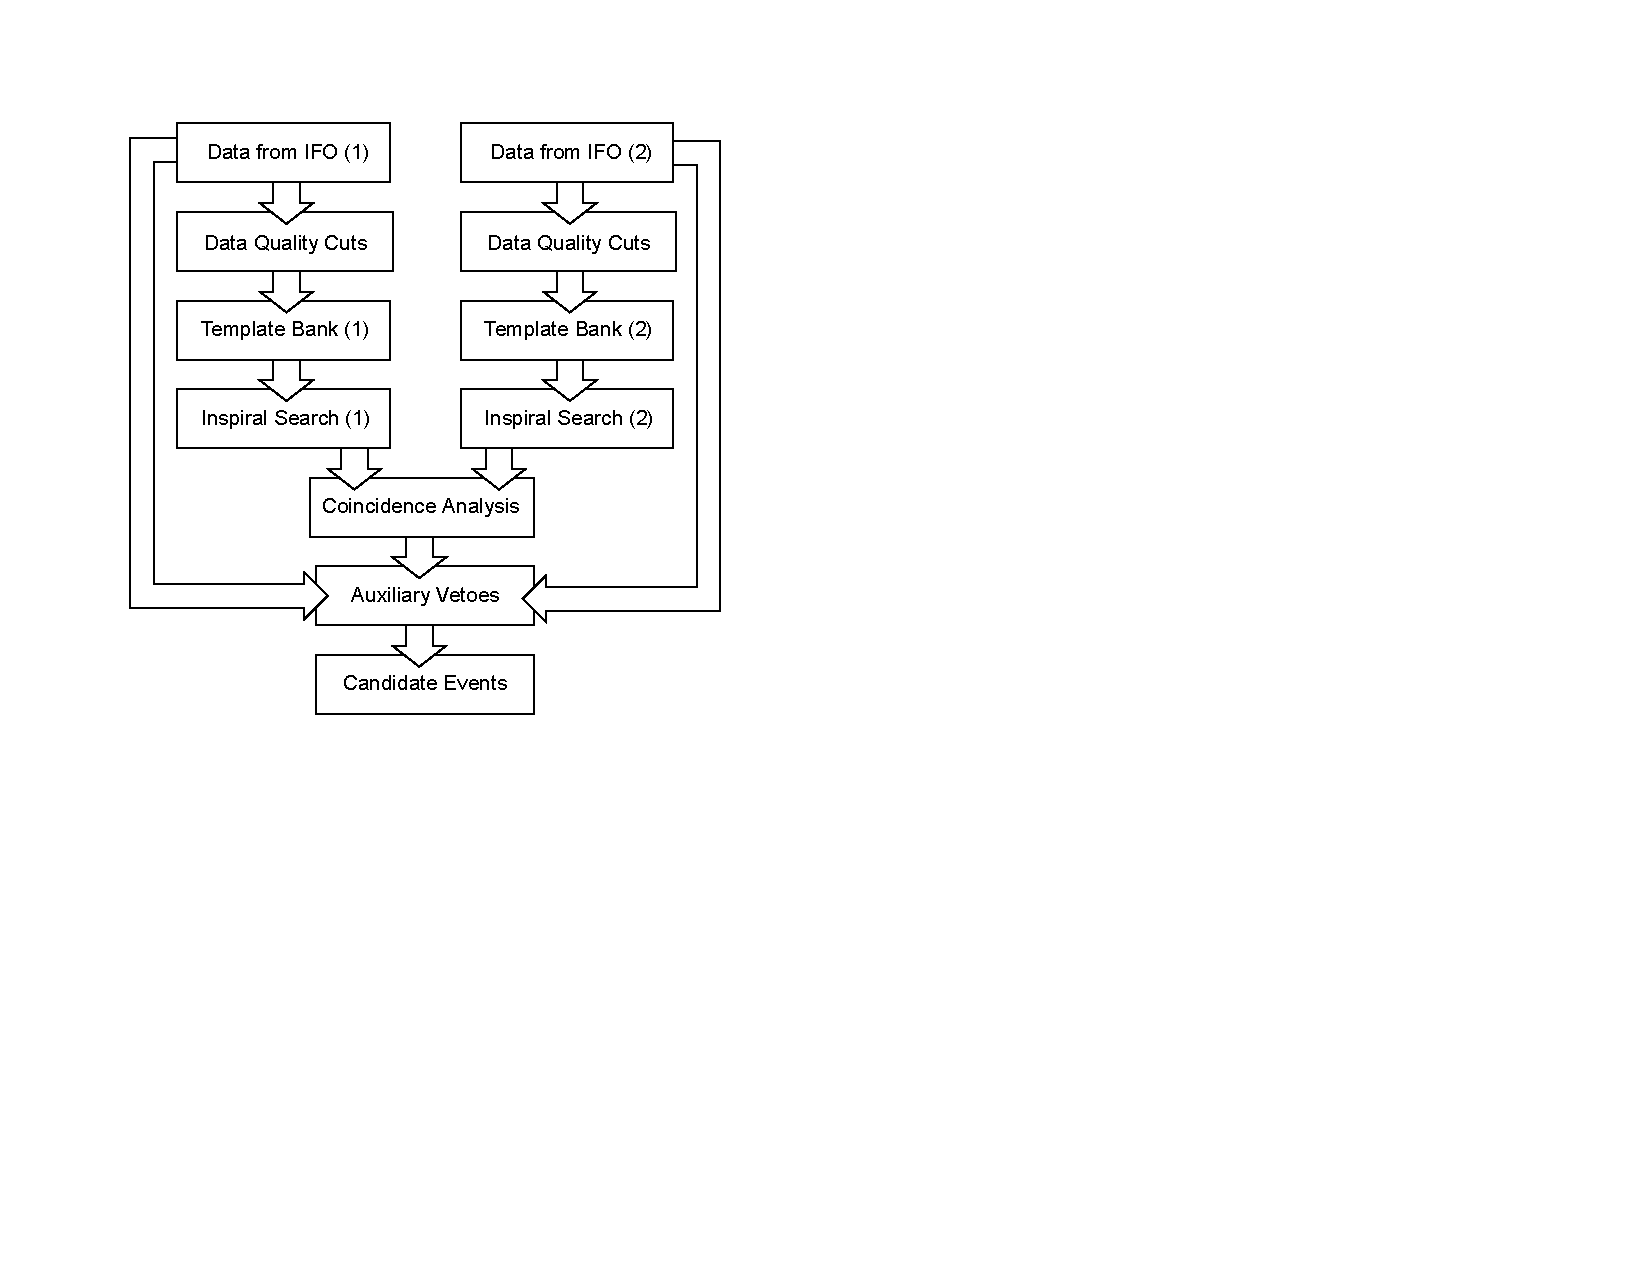
\includegraphics[height=0.6\textheight]{figures/pipeline/simple_pipe}
\end{center}
\caption[Simple Pipeline to Search Data From Two Interferometers]{
A simple pipeline used to search data from two interferometers for inspiral
signals. Raw data from interferometer, labeled $1$ and $2$, is recorded at the
observatories. Data quality cuts are then applied to the raw data to discard
times when the interferometer was not in a stable operating mode. Power
spectra generated from the data are used to generate a template bank for the
inspiral population being searched for. The template banks and interferometer
data are used to generate inspiral triggers for each interferometer. The
triggers for each interferometer are tested for coincidence, as a true
inspiral signal should be present in both interferometers at the same time, up
to the time it takes a gravitational wave to travel between the observatories.
Other coincidence tests, such as waveform parameter consistency, can be
applied at this stage. Transient noise sources may be detected in auxiliary
interferometer channels, for example seismometers. Such channels may be used to 
veto triggers that survive the coincidence analysis but are coincident with
the signature of noise in the auxiliary channel. Finally we obtain a sample of
candidate events for further investigation. Each step of the pipeline has many
parameters that can be tuned to minimize the false alarm and false dismissal 
rates.  
}
\end{figure}

\begin{figure}[p]
\label{f:s1loudest}
\begin{center}
\begin{tabular}{cc}
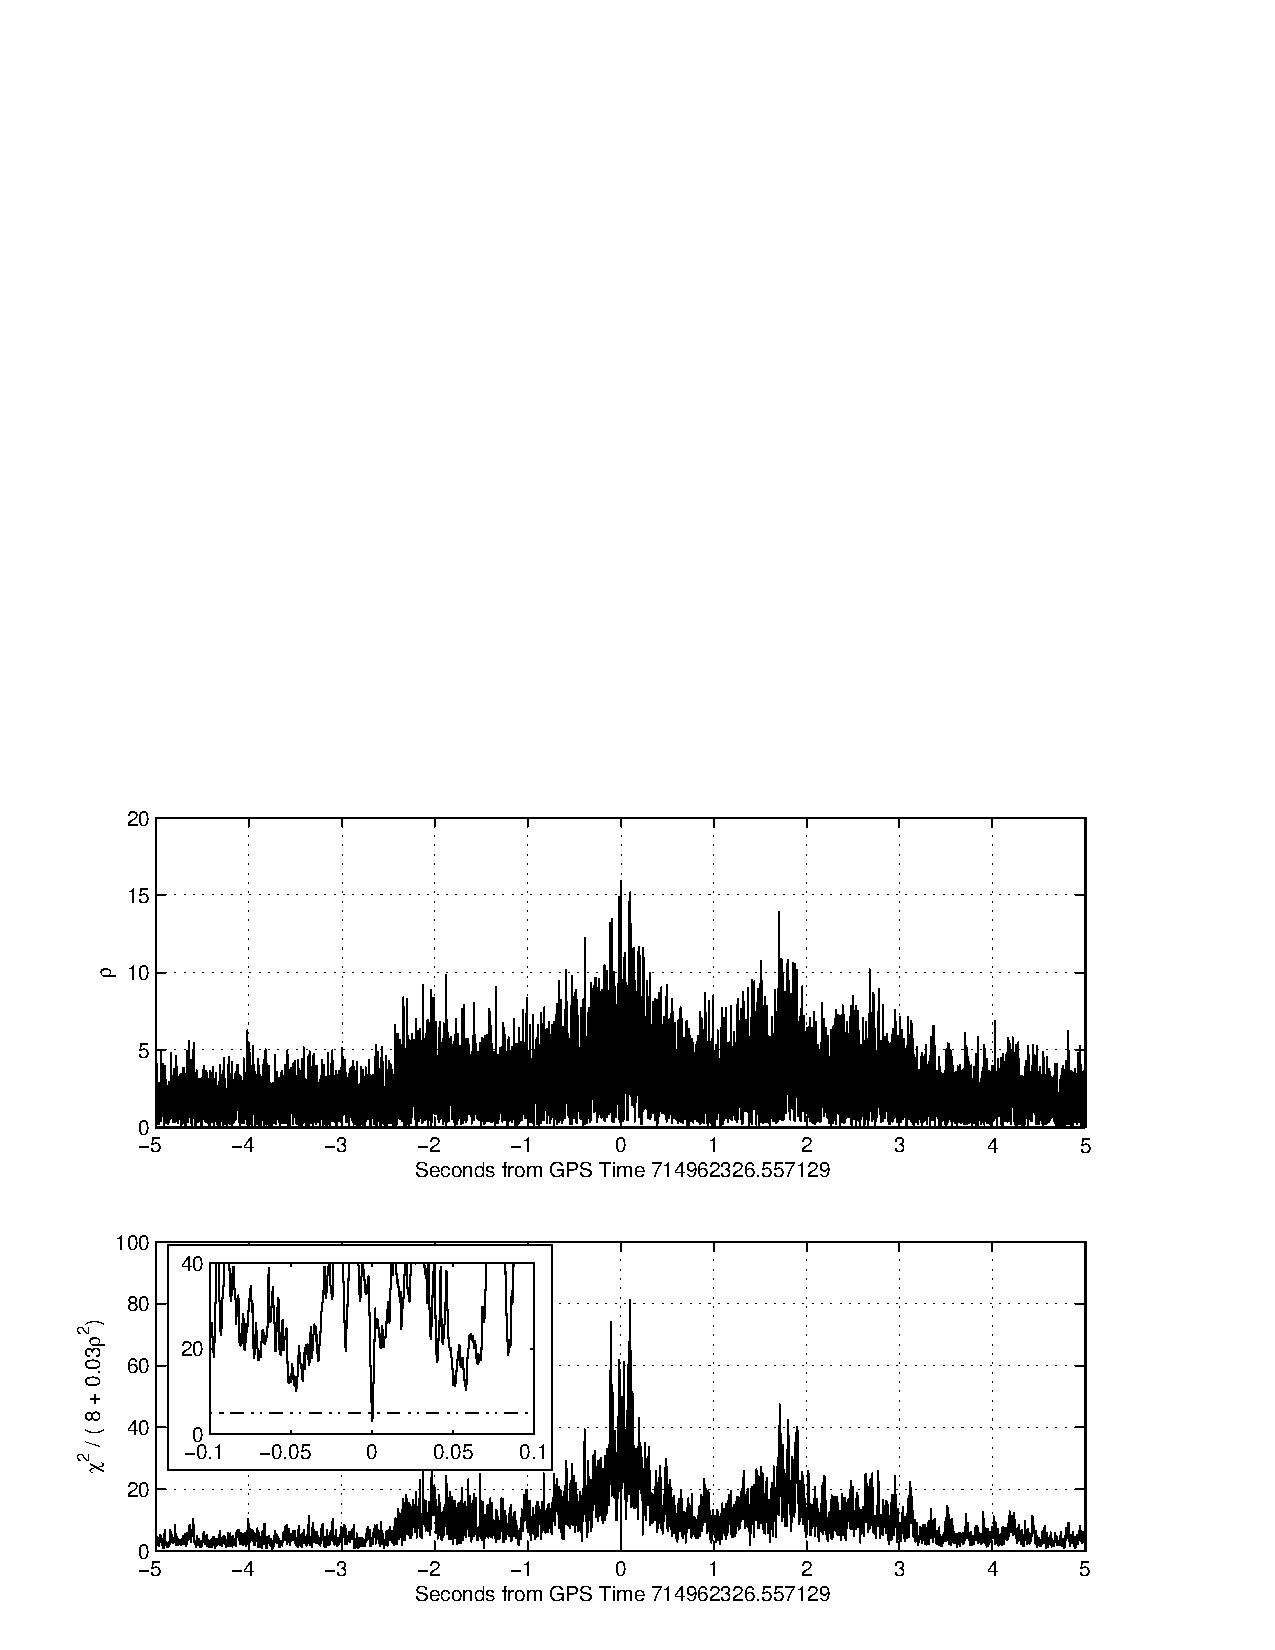
\includegraphics[width=0.475\linewidth]{figures/pipeline/loudest-snrplot} &
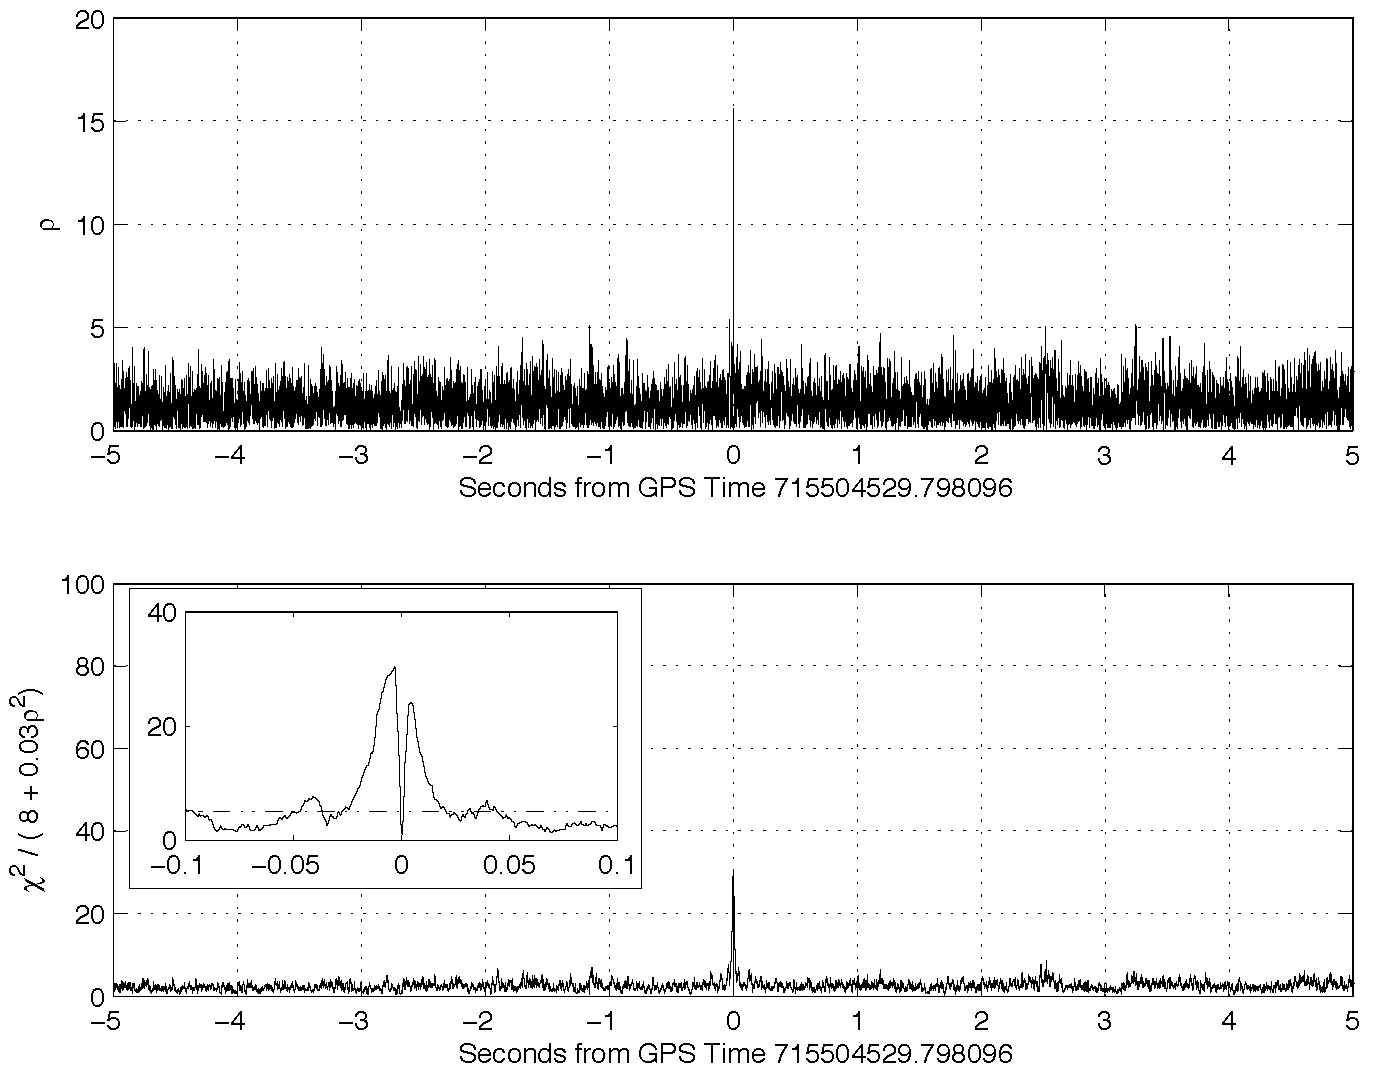
\includegraphics[width=0.475\linewidth]{figures/pipeline/injection-snrplot}\\
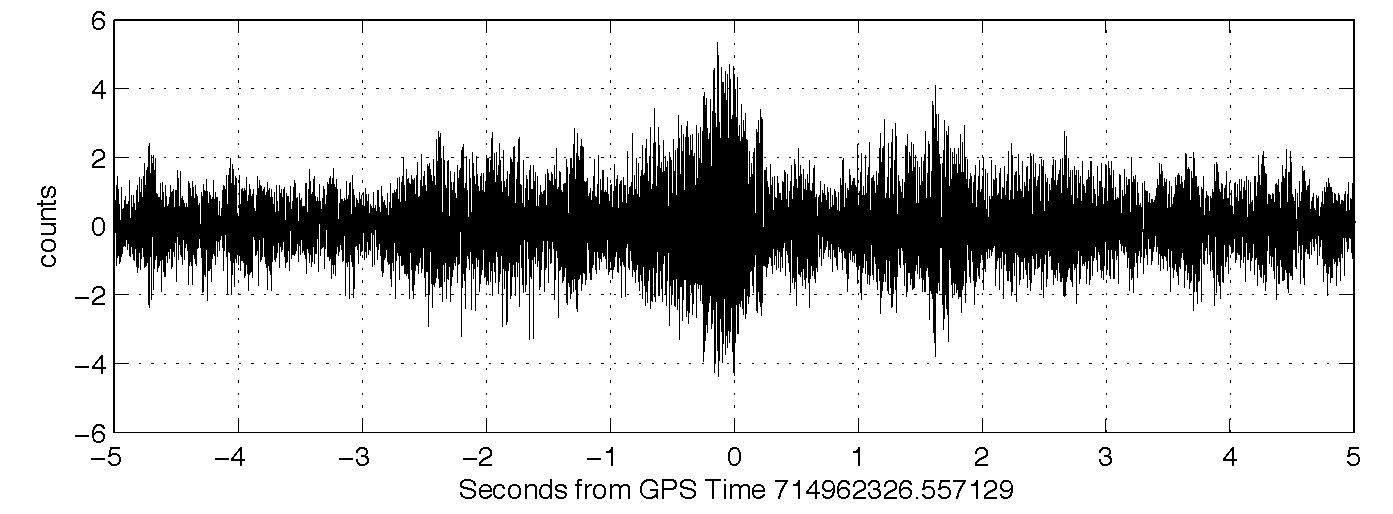
\includegraphics[width=0.475\linewidth]{figures/pipeline/loudest-ts} &
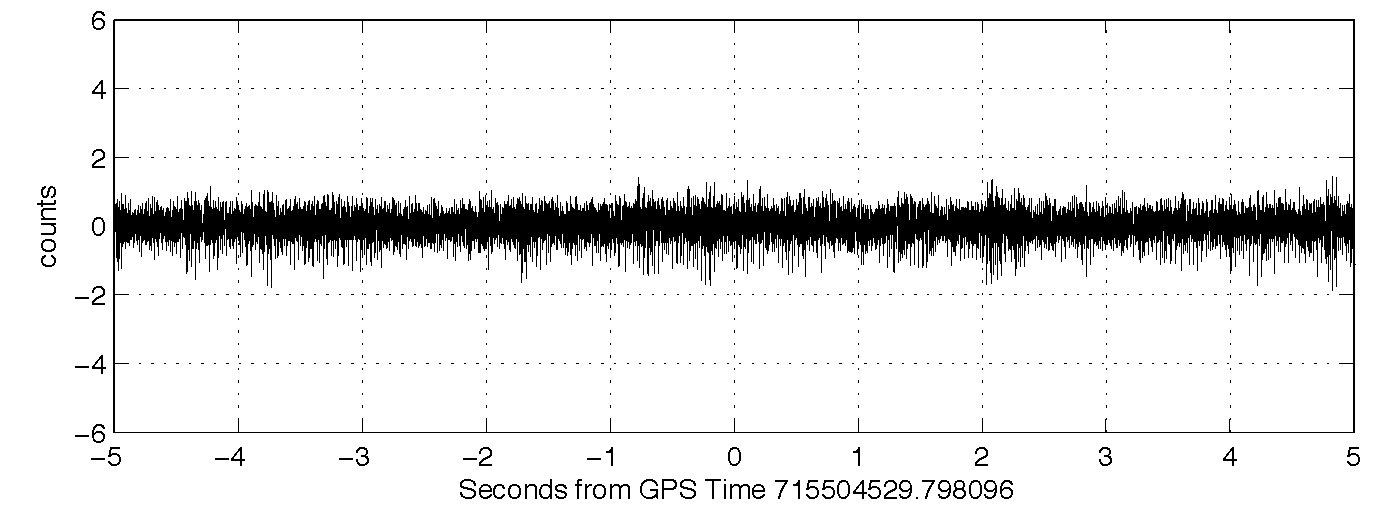
\includegraphics[width=0.475\linewidth]{figures/pipeline/injection-ts}
\end{tabular}
\end{center}
\caption[Largest Inspiral Trigger Seen in the S1 Analysis]{
Left Panels: The largest signal-to-noise ratio candidate event seen during the
search of the LIGO S1 data. The top panel shows the signal-to-noise time
series, $\rho(t)$.  Notice that $\rho(t)$ is greater than the S1 threshold of
$6.5$ many times in a  $\sim 5$ second interval around the candidate event.
The center panel shows $\chi^2/ (p+ \delta^2 \rho^2)$ as a function of time
for the values of $\delta^2 = 0.03$ and $p = 8$ used in S1.  Notice $\chi^2 /
(p+ 0.03 \rho^2)$ is greater than the threshold of $5$ for $\sim 5$ seconds
around the candidate event,  but drops below this threshold right at the time
of maximum $\rho$.  The inset shows this more clearly for $\pm 0.1$ second
around the event where the threshold is indicated by a dot-dashed horizontal
line.  The bottom panel shows the time series for this candidate event after
applying a high-pass filter with a knee frequency of 200~Hz.  Notice the
bursting behavior which does not look like an inspiral chirp signal.  \break
Right Panels: A simulated injection into the L1 data.  This example was chosen
for comparison with the largest signal-to-noise ratio event shown in the left
panels since it similar in mass parameters, detected signal to noise and
$\chi^2$.   The instrument was behaving well at the time around the simulated
injection.  The top panel shows that $\rho(t) < 6.5$ except in close proximity
to the signal detection time.  The center panel shows $\chi^2/ (p+ 0.03
\rho^2)$ as a function of time.  Notice that it is much closer to threshold at
all times around the simulated injection; this contrasts dramatically with the
case of the candidate event shown in the left panels.  The inset shows this
more clearly for $\pm 0.1$ seconds around the injection.  The bottom panel
shows the time series for this simulated injection after applying a high-pass
filter with a knee frequency of 200~Hz.  The inspiral chirp signal is not
visible in the noisy detector output.
}
\end{figure}

\begin{table}[p]
\label{t:dqflags}
\begin{center}
\begin{tabular}{ll}
Mandatory Data Quality Cut & Description \\\hline
OUTSIDE\_S2   &Data is outside of official S2 time interval \\
MISSING\_RAW  &Raw data is missing \\
DAQ\_DROPOUT       & Dropout in data acquisition system \\
MISSING\_RDS       & Data is unavailable for analysis \\
INVALID\_TIMING    & Timing believed to be unreliable \\
CALIB\_LINE\_NO\_RDS\_V03 & Problem with accessing data for calibration \\
DAQ\_REBOOT               & One or more data acquisition system rebooted \\
INVALID\_CALIB\_LINE  & Problem with calibration line strength \\
NO\_CALIB                 & Calibration line turned off \\
LOW\_CALIB                & Calibration line strength too low \\
\hline\hline
\\
Discretionary Data Quality Cut & Description \\\hline
MICH\_FILT    &One or more Michelson control loop \\
&filters was not in its nominal state \\
AS\_PD\_SATURATION & Antisymmetric port photodiode saturated \\
ASQ\_LARGEP2P      & Large peak-to-peak range seen in AS\_Q \\
&at end of lock \\
NONSTAND\_CTRLS    & Non-standard controls affecting calibration\\
&and couplings \\
ASQ\_OUTLIER\_CLUSTER     & Cluster of large AS\_Q outliers \\
&in short time interval \\
ASQ\_OUTLIER\_CORRELATED  & Large ASQ outliers correlated with \\
&outliers in auxiliary IFO channel \\
ASQ\_LOWBAND\_OUTLIER     & High noise below 100 Hz in AS\_Q \\
ASQ\_UPPERBAND\_OUTLIER   & High noise in 100-7000 Hz in AS\_Q \\
\hline\hline
\end{tabular}
\end{center}
\caption[Data Quality Cuts Available During S2]{%
Data quality cuts available during the S2 science run and their meanings. 
Some data quality flags monitor human error in the operation of the
instrument that make the data unsuitable for analysis, such as NO\_CALIB and
NONSTAND\_CTRLS. Others cuts identify hardware or software failures in the
operation of the instrument, for example MISSING\_RAW and DAQ\_REBOOT.
Additional cuts like AS\_PD\_SATURATION and ASQ\_UPPERBAND\_OUTLIER monitor
the gravitational wave channel, AS\_Q, for unusable data.
}
\end{table}

\begin{figure}[p]
\label{f:snr_resample_loss}
\begin{center}
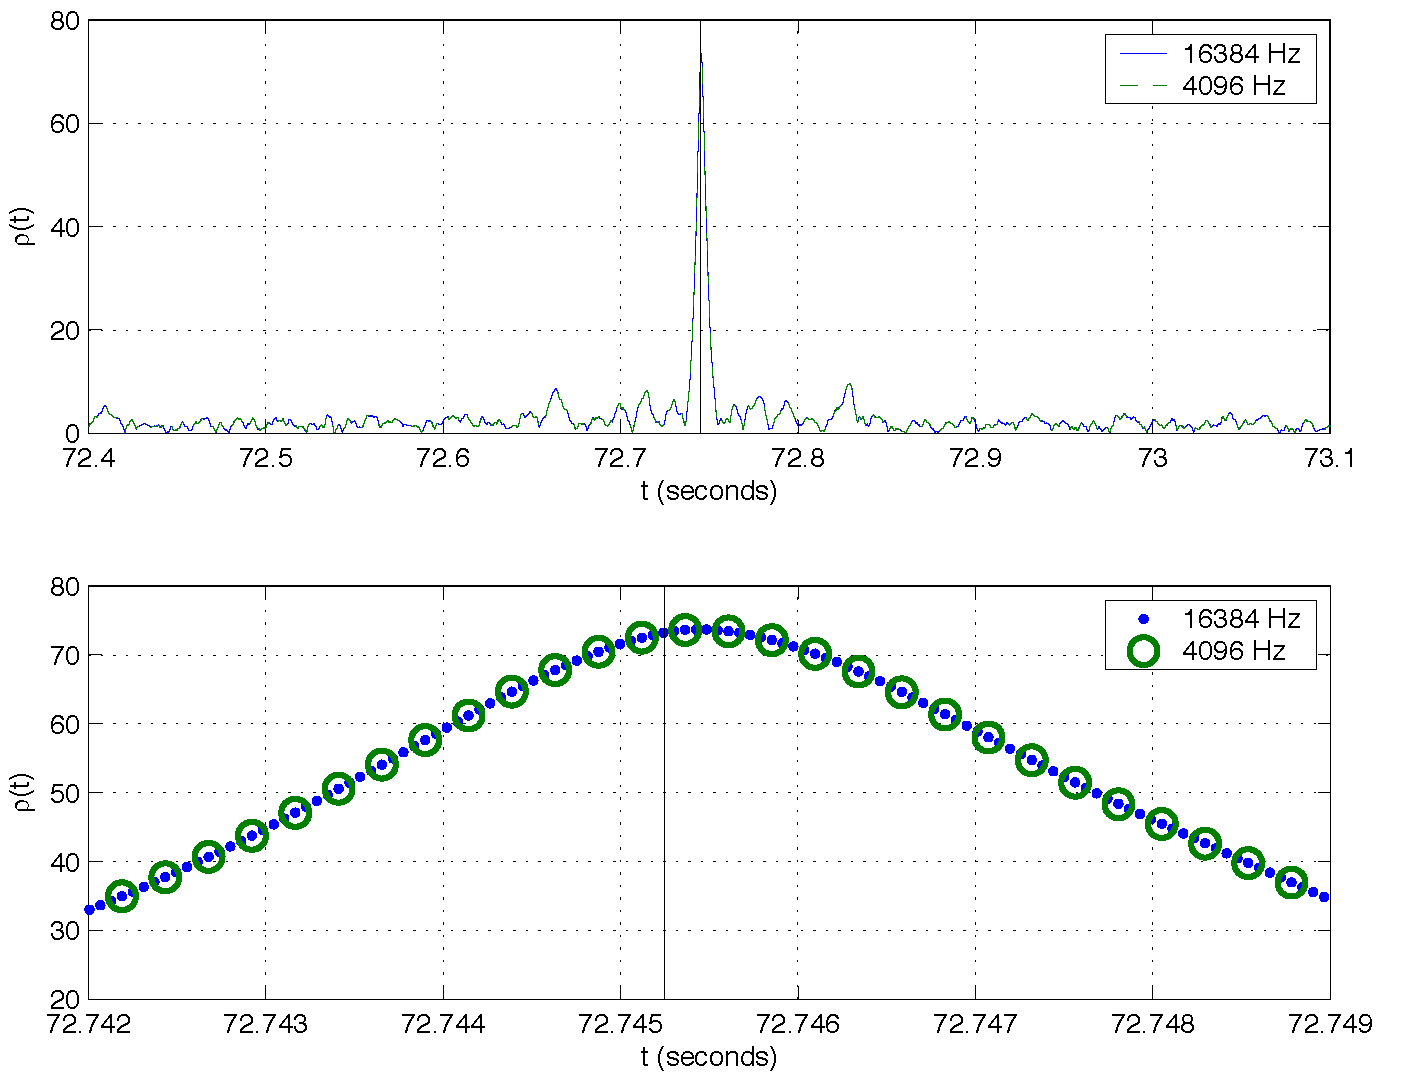
\includegraphics[width=\linewidth]{figures/pipeline/snr_resample_loss}
\end{center}
\caption[Loss in Signal-to-noise Ratio Due to Resampling]{%
The loss in signal-to-noise ratio for a $0.2,0.2\, M_\odot$ black hole
MACHO binary due to resampling. The inspiral waveform is generated at
$16\,384$~Hz and injected into data with a typical S2 noise curve. The end
time of the waveform is at $72.74525$~seconds, shown by the vertical line in
both plots. The top panned shows the signal-to-noise ratio for the data
segment when using data at the full bandwidth and data resampled to 
$4096$~Hz. The bottom panel shows the same data close to the end time of the
injection. The loss in signal-to-noise ratio for the inspiral trigger 
generated at $4096$~Hz is $0.1\%$.
}
\end{figure}

\begin{figure}[p]
\label{f:s2_segments}
\begin{center}
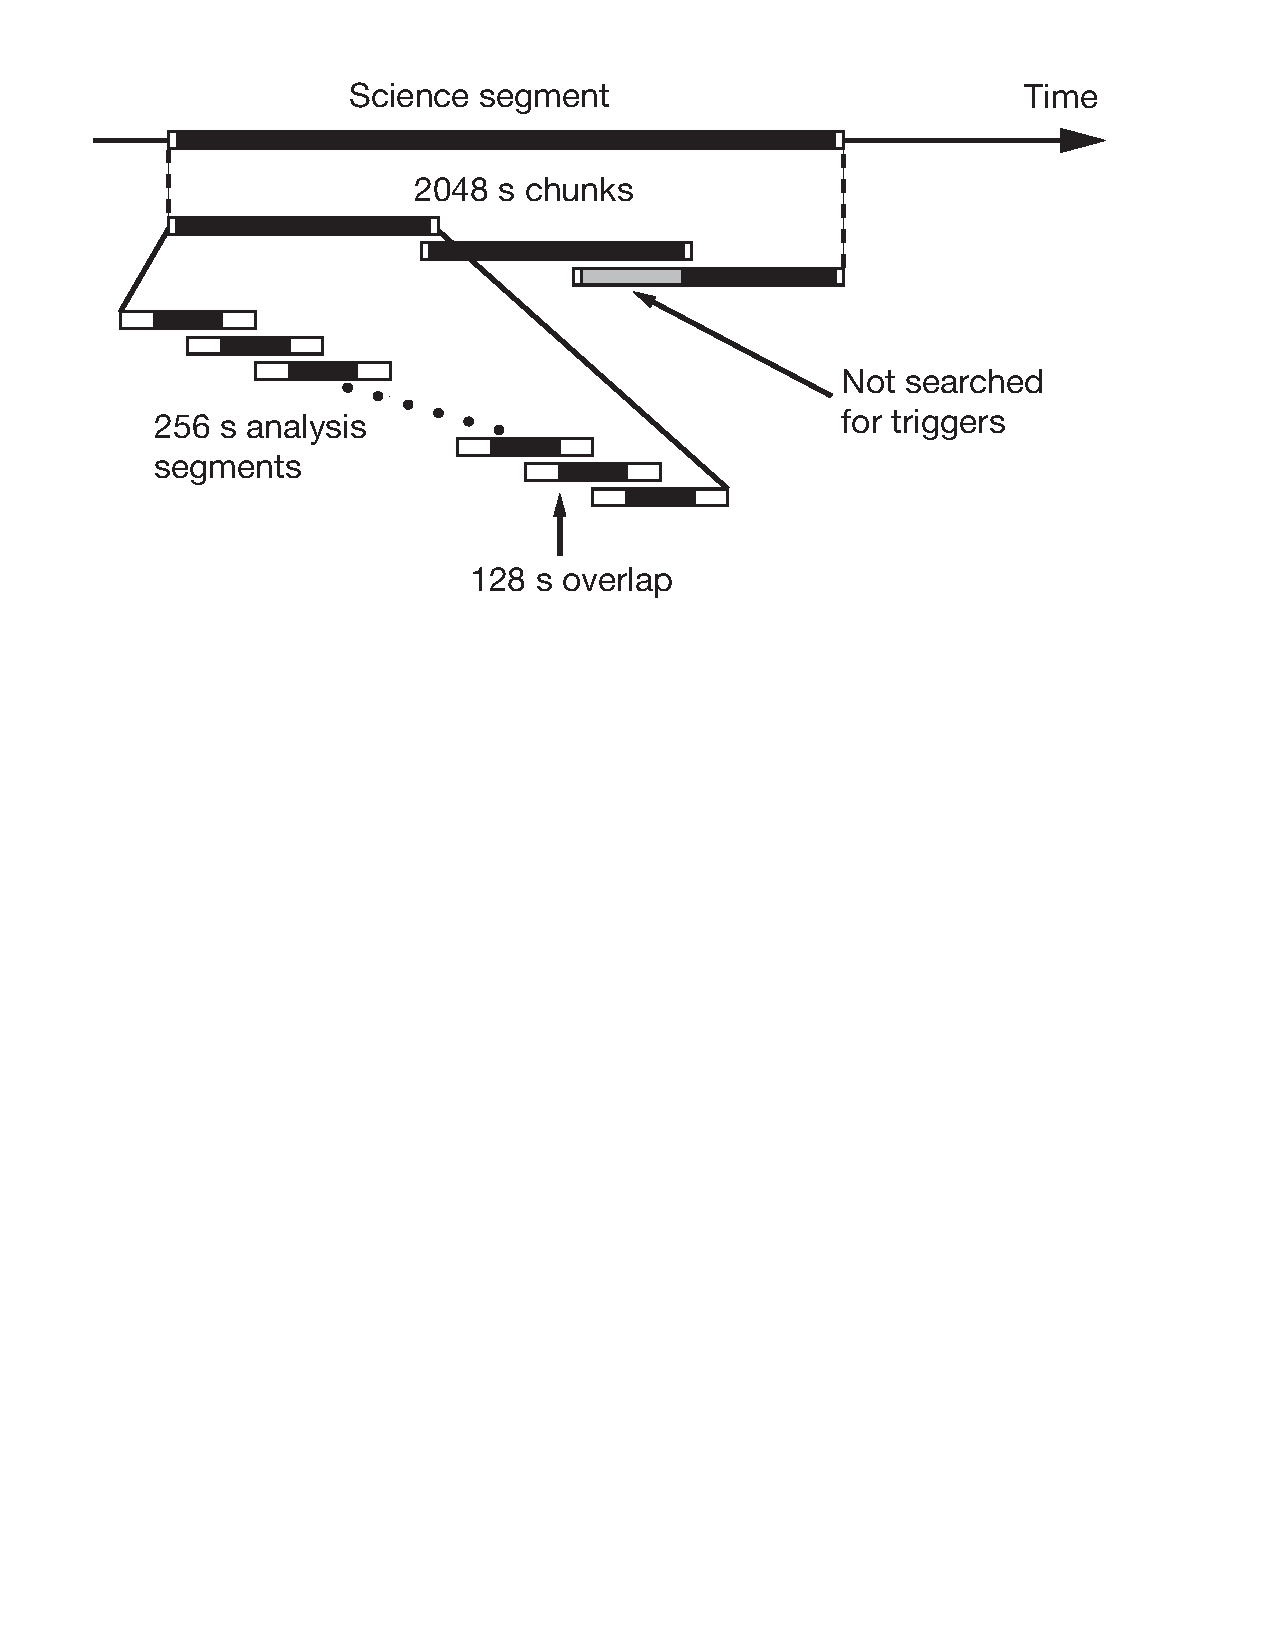
\includegraphics[width=\linewidth]{figures/pipeline/s2_segments}
\end{center}
\caption[Algorithm Used to Divide Science Segments into Data Analysis
Segments]{%
The algorithm used to divide science segments into data analysis segments.
Science segments are divided into $2048$~s chunks overlapped by $128$~s.
(Science segments shorter than $2048$~s are ignored.) An additional chunk with
a larger overlap is added to cover any remaining data at the end of a science
segment.  Each chunk is divided into $15$ analysis segments of length $256$~s
for filtering. The first and last $64$~s of each analysis segment is ignored,
so the segments overlap by $128$~s.  Areas shaded black are filtered for
triggers by the search pipeline. The gray area in the last chunk of the
science segment is not searched for triggers as this time is covered by the
preceding chunk, however this data is used in the PSD estimate for the final
chunk.
}
\end{figure}

\begin{figure}[p]
\label{f:s2_banks}
\begin{tabular}{c}
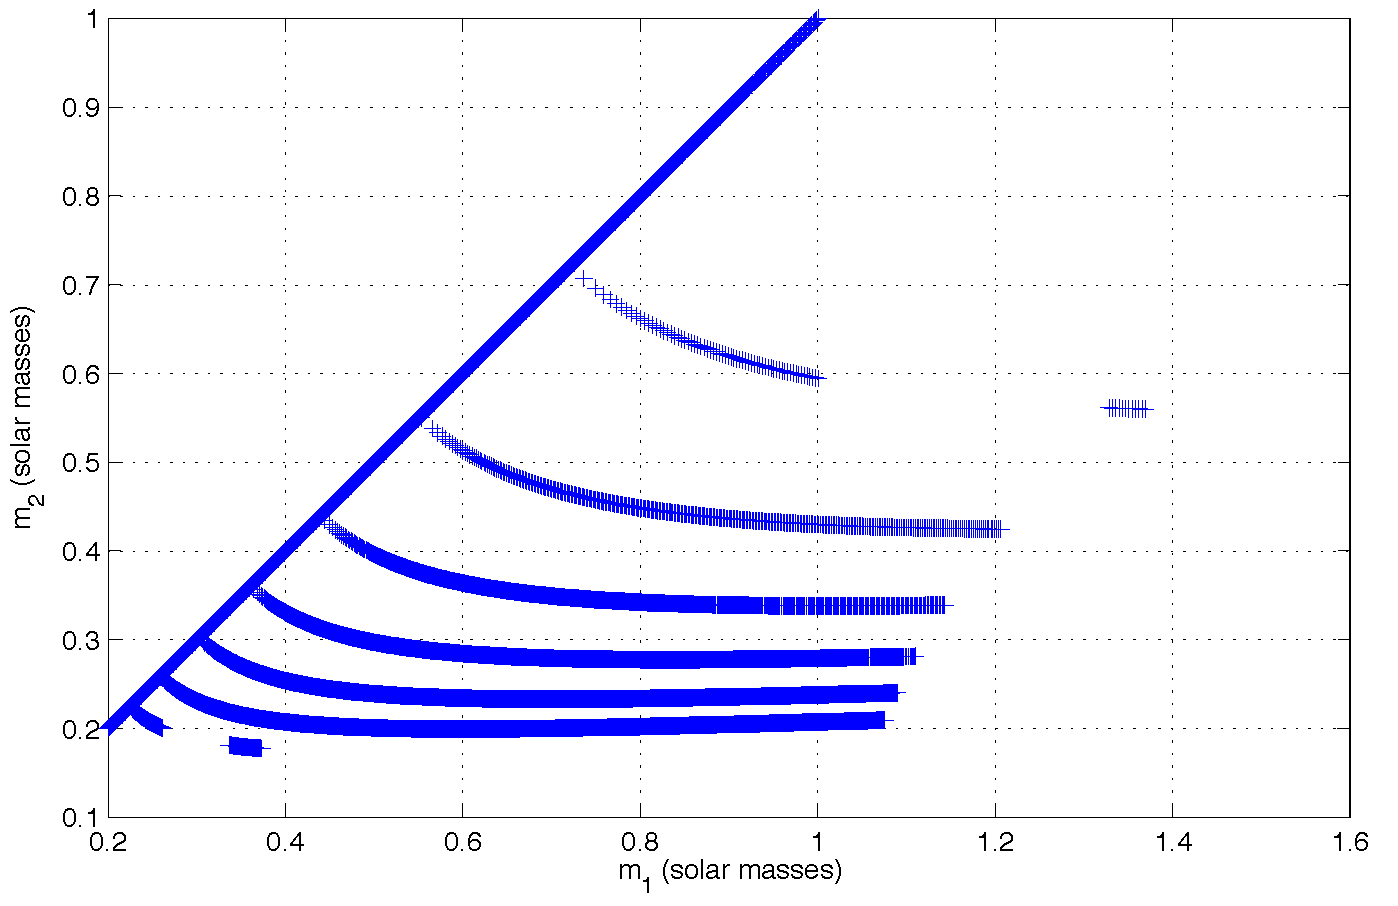
\includegraphics[width=\linewidth]{figures/pipeline/macho_bank}
\end{tabular}
\caption[Binary Black Hole MACHO Template Bank]{
The template bank required to cover the binary black hole MACHO parameter
space from $0.2$ to $1$ $M_\odot$ at a minimal match of $95\%$.  The template
bank is generated from the average power spectral density of a typical S2
analysis chunk (starting at GPS time 734256712.) The large number of
templates in the BBHMACHO bank is due to the lager number of cycles of the
MACHO templates in the sensitive band of the interferometer. The placement of
templates outside the mass parameter space is required to ensure that any
signal that lies in the space has a minimal match $> 0.95$.
}
\end{figure}

\begin{figure}[p]
\label{f:gmst_dist_ratio}
\vspace{5pt}
\begin{center}
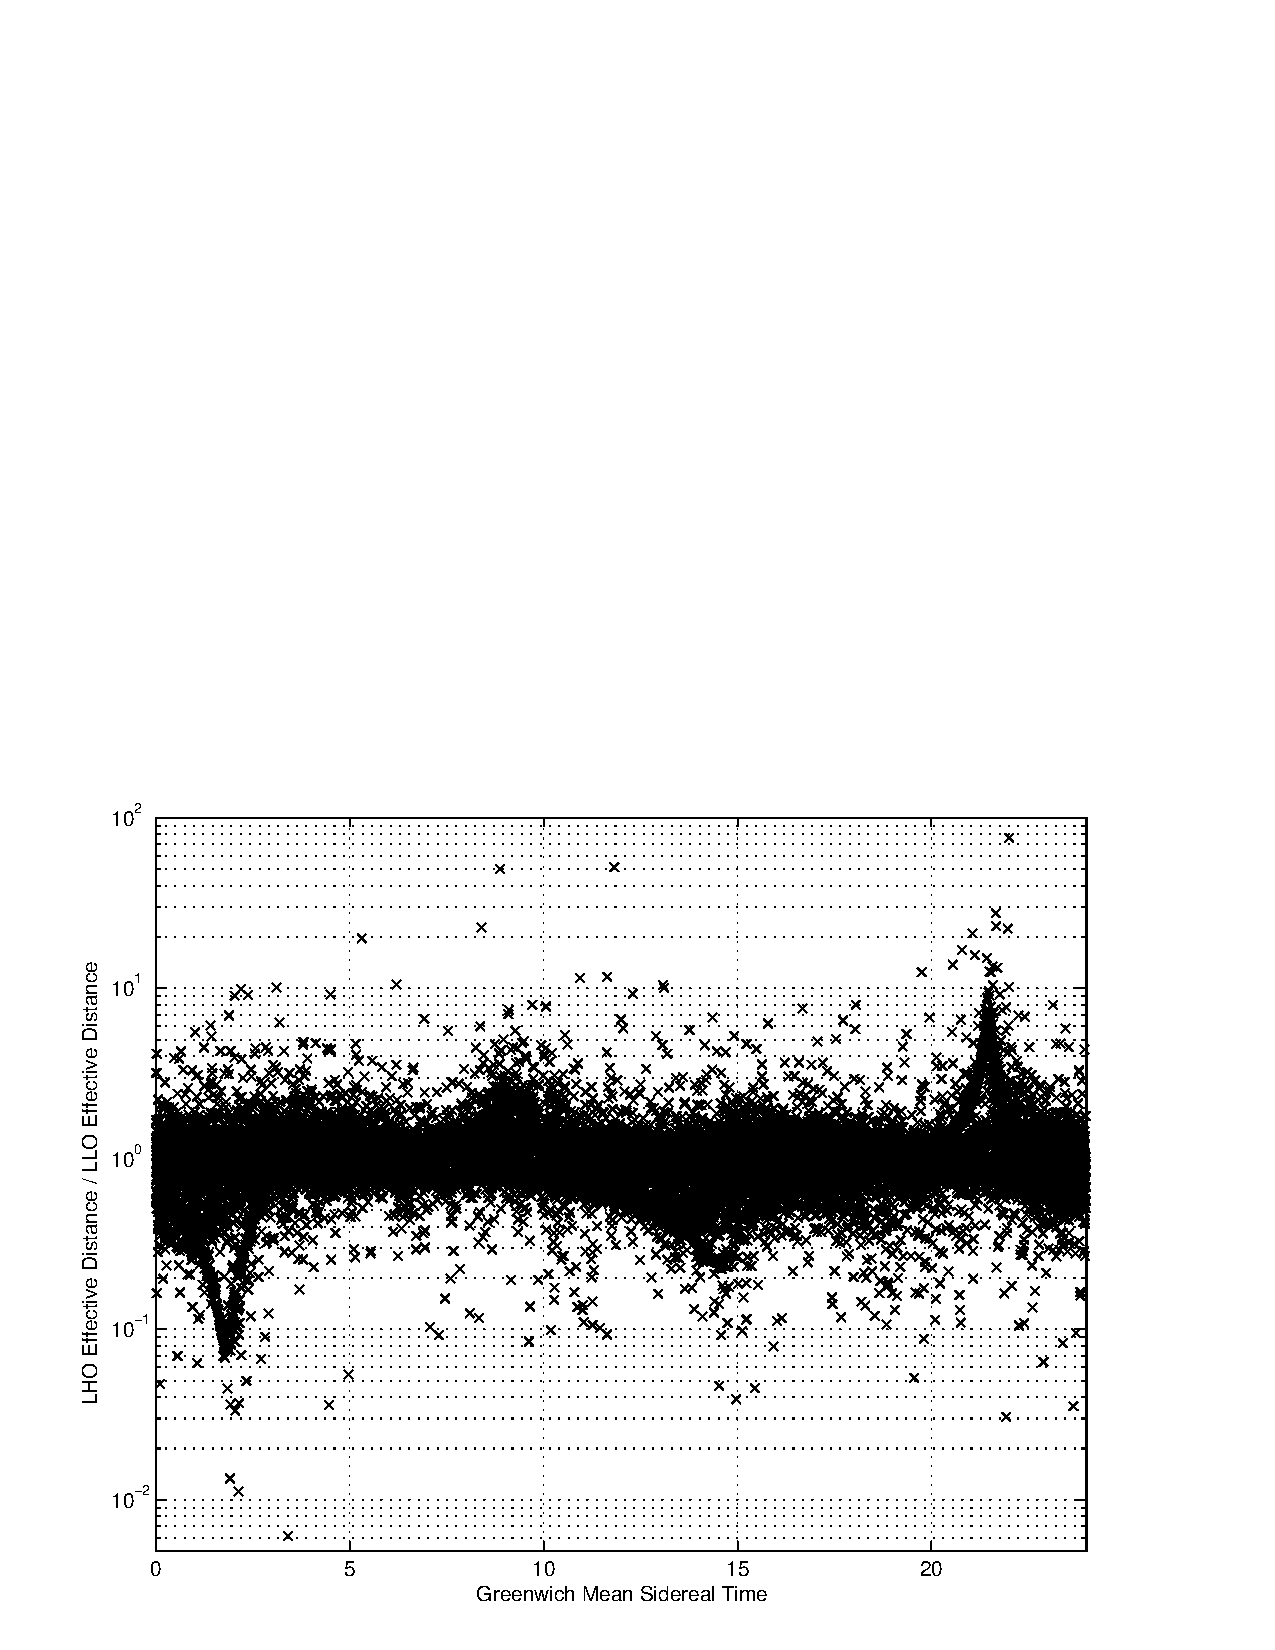
\includegraphics[width=\linewidth]{figures/pipeline/gmst_dist_ratio}    
\end{center}
\caption[Ratio of Effective Distance of Injected Signals Between Observatories]{%
The ratio of the known effective distance of an injected signal in the Hanford
Observatory (LHO) to the known effective distance of an injected signal in the
Livingston Observatory (LLO) as a function of Greenwich Mean Sidereal Time.
The slight misalignment of the interferometers at the two different
observatories due to the curvature of the earth causes the antenna pattern of
the detectors to differ. As a result the distance at which a binary system
appears is different in each detector, even in the absence of noise.  The
ratio of effective distances can be significant, so this precludes the use of
an amplitude cut when testing for inspiral trigger coincidence between
different observatories.
}
\end{figure}

\begin{figure}[p]
\label{f:coinc_test}
\begin{center}
\hspace*{-0.2in}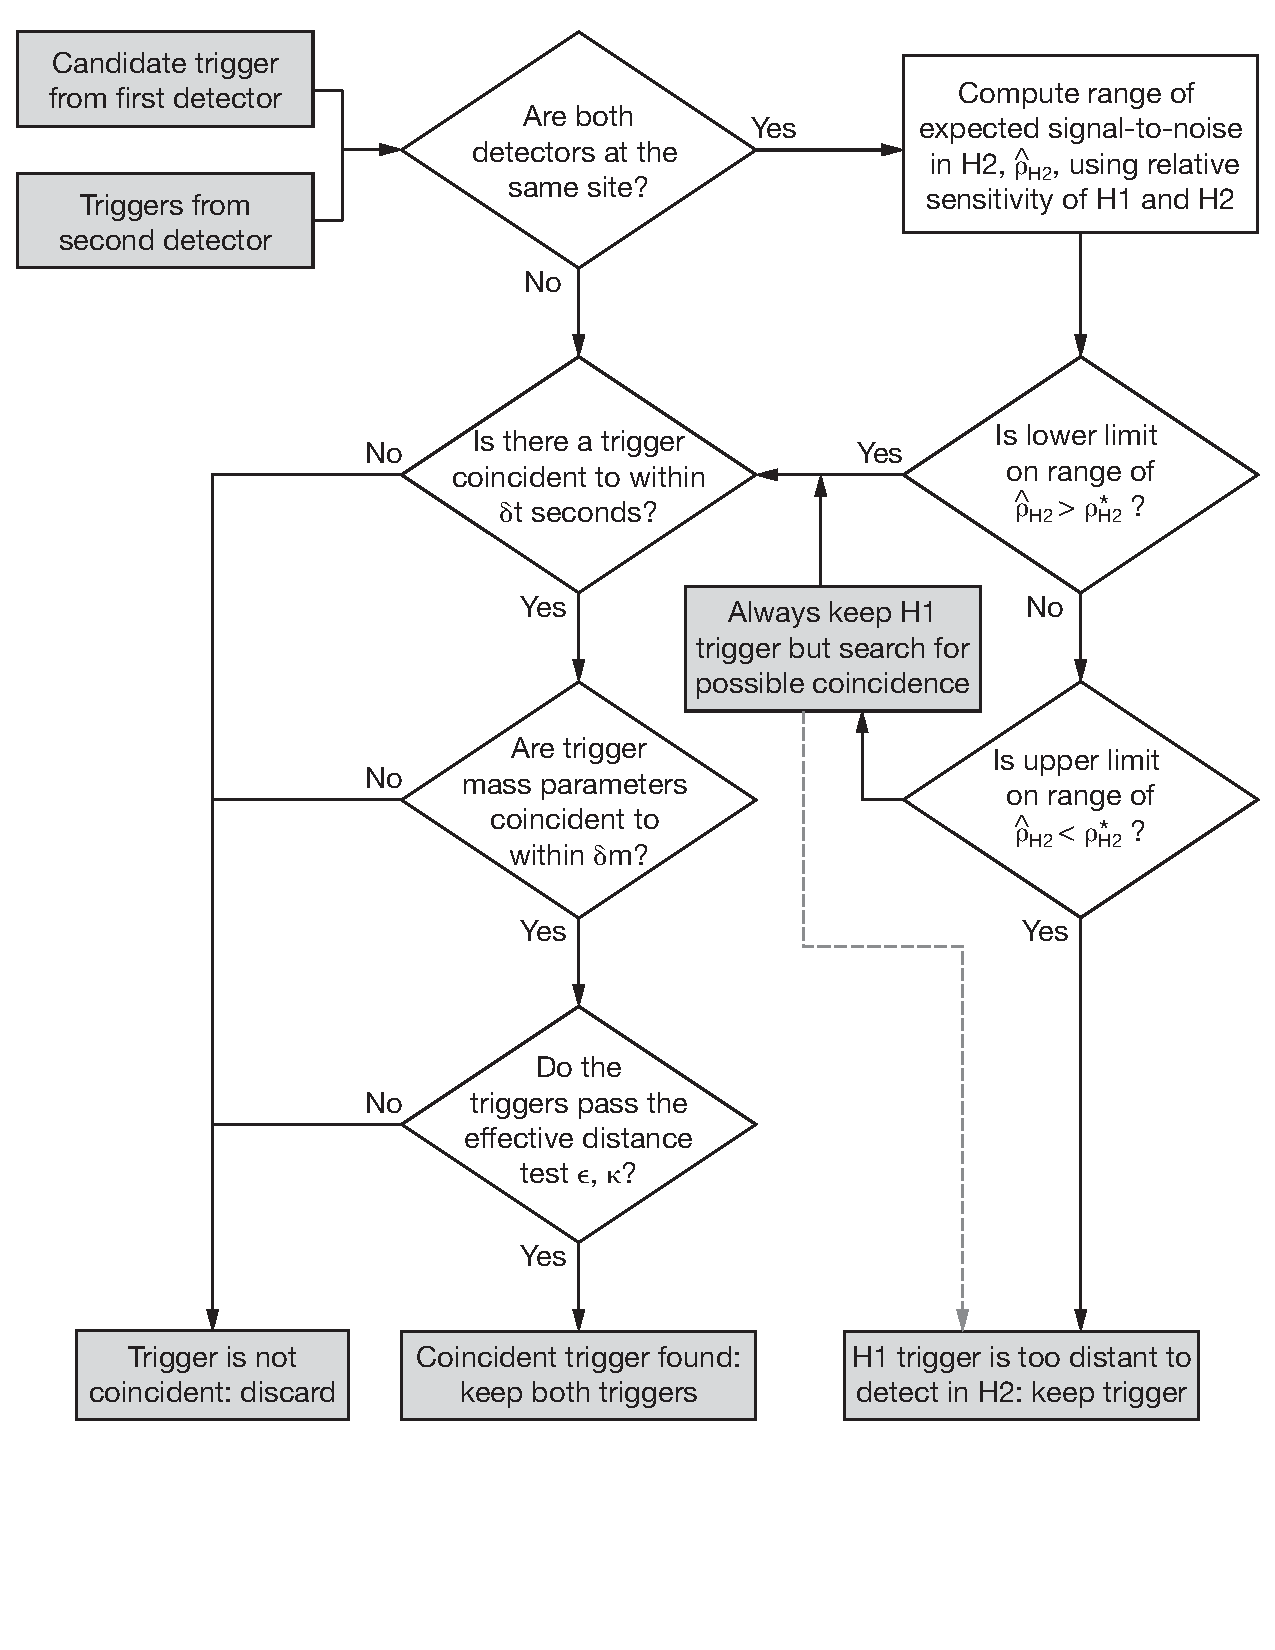
\includegraphics[width=\linewidth]{figures/pipeline/s2_coinc_test}
\end{center}
\caption[Trigger Coincidence Test]{%
The test to decide if a trigger in the first detector has a coincident 
trigger in the second detector. If detectors are at different sites, time and
mass coincidence are demanded. The effective distance cut is disabled by 
setting $\kappa = 1000$. If the detectors are at the same site, we ask if the
maximum distance to which H2 can see at the signal-to-noise threshold
$\rho_\mathrm{H2}^\ast$ is greater than the distance of the H1 trigger,
allowing for errors in the measurement of the trigger distance. If this is the
case, we demand time, mass and effective distance coincidence.  If distance to
which H2 can see overlaps the error in measured distance of the H1 trigger, we
search for a trigger in H2, but always keep the H1 trigger even if no
coincident trigger is found. If the minimum of the error in measured distance
of the H1 trigger is greater than the maximum distance to which H2 can detect
a trigger we keep the H1 trigger without searching for coincidence.}
\end{figure}

\begin{figure}[p]
\label{f:vetoes}
\vspace{5pt}
\begin{center}
\begin{tabular}{cc}
(i) & (ii) \\
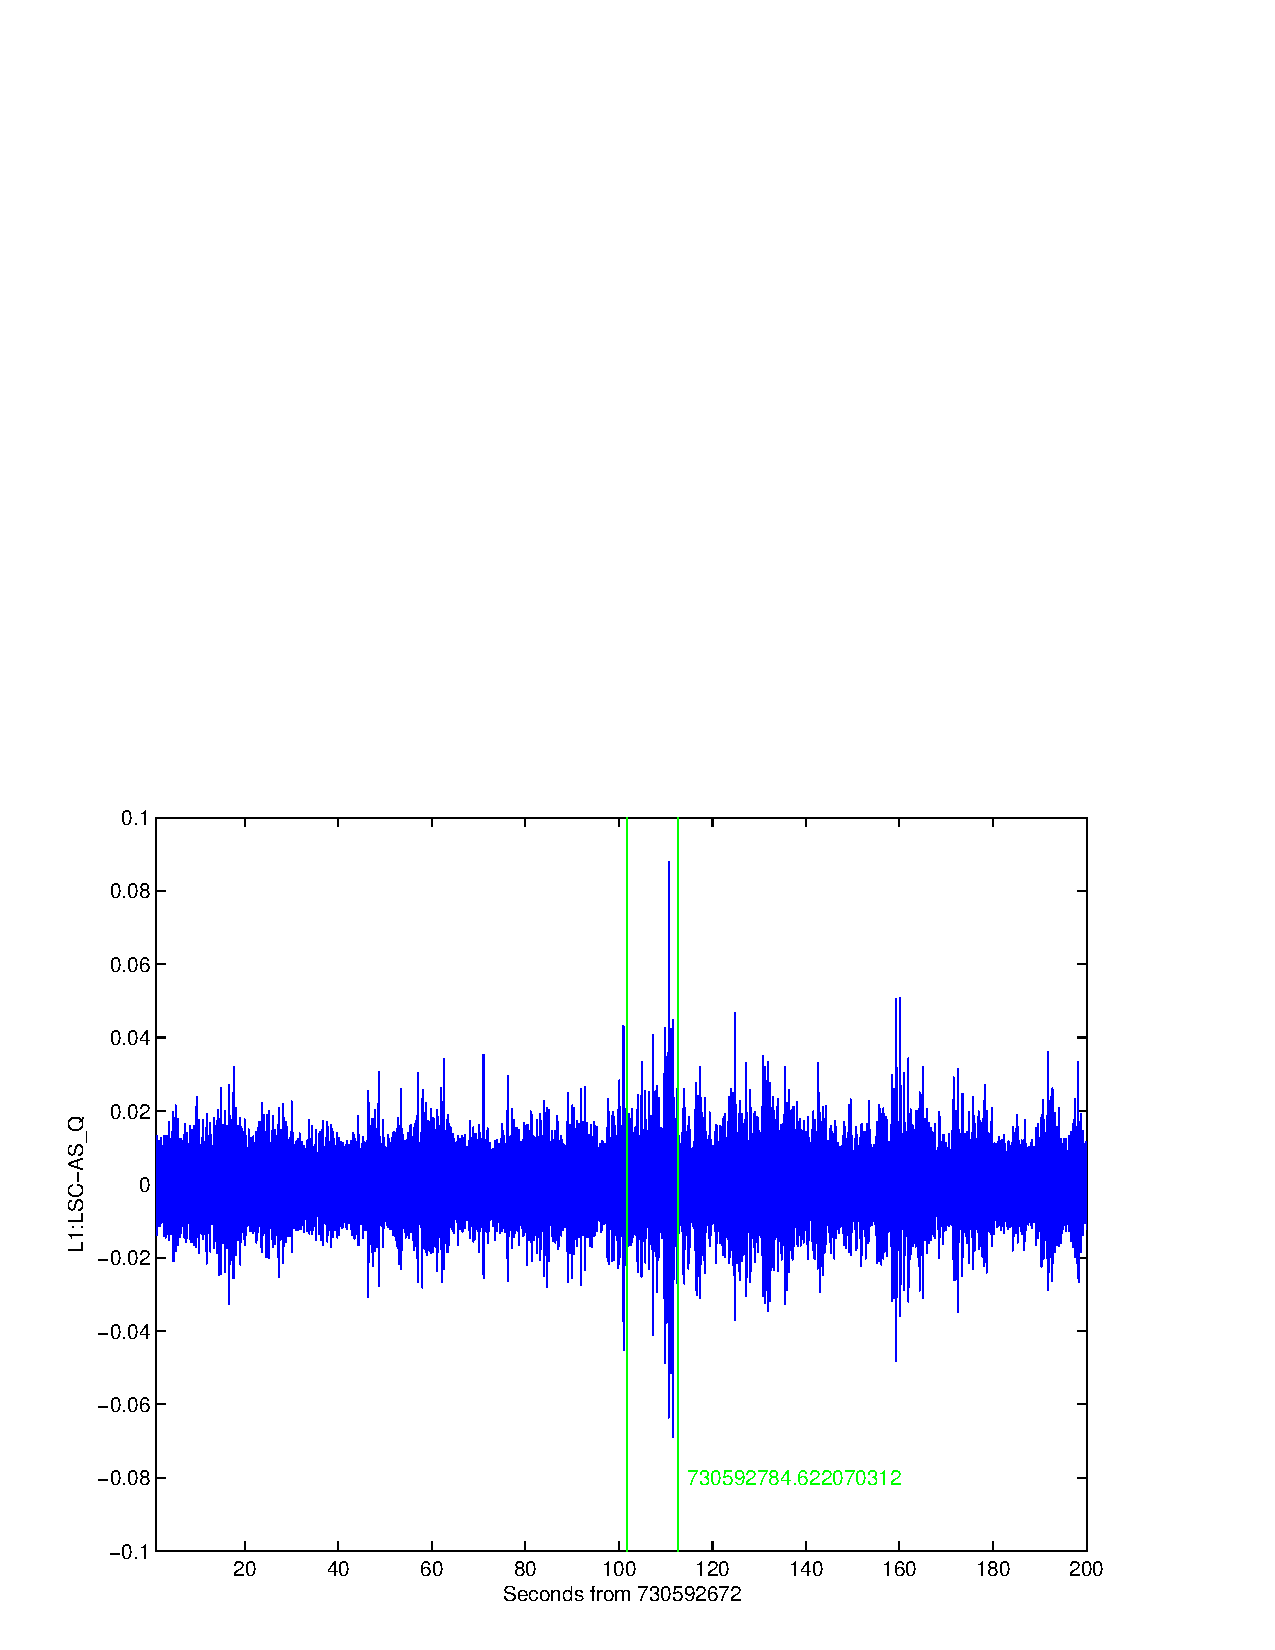
\includegraphics[width=0.475\linewidth]{figures/pipeline/trigger_730592784_as_q} &
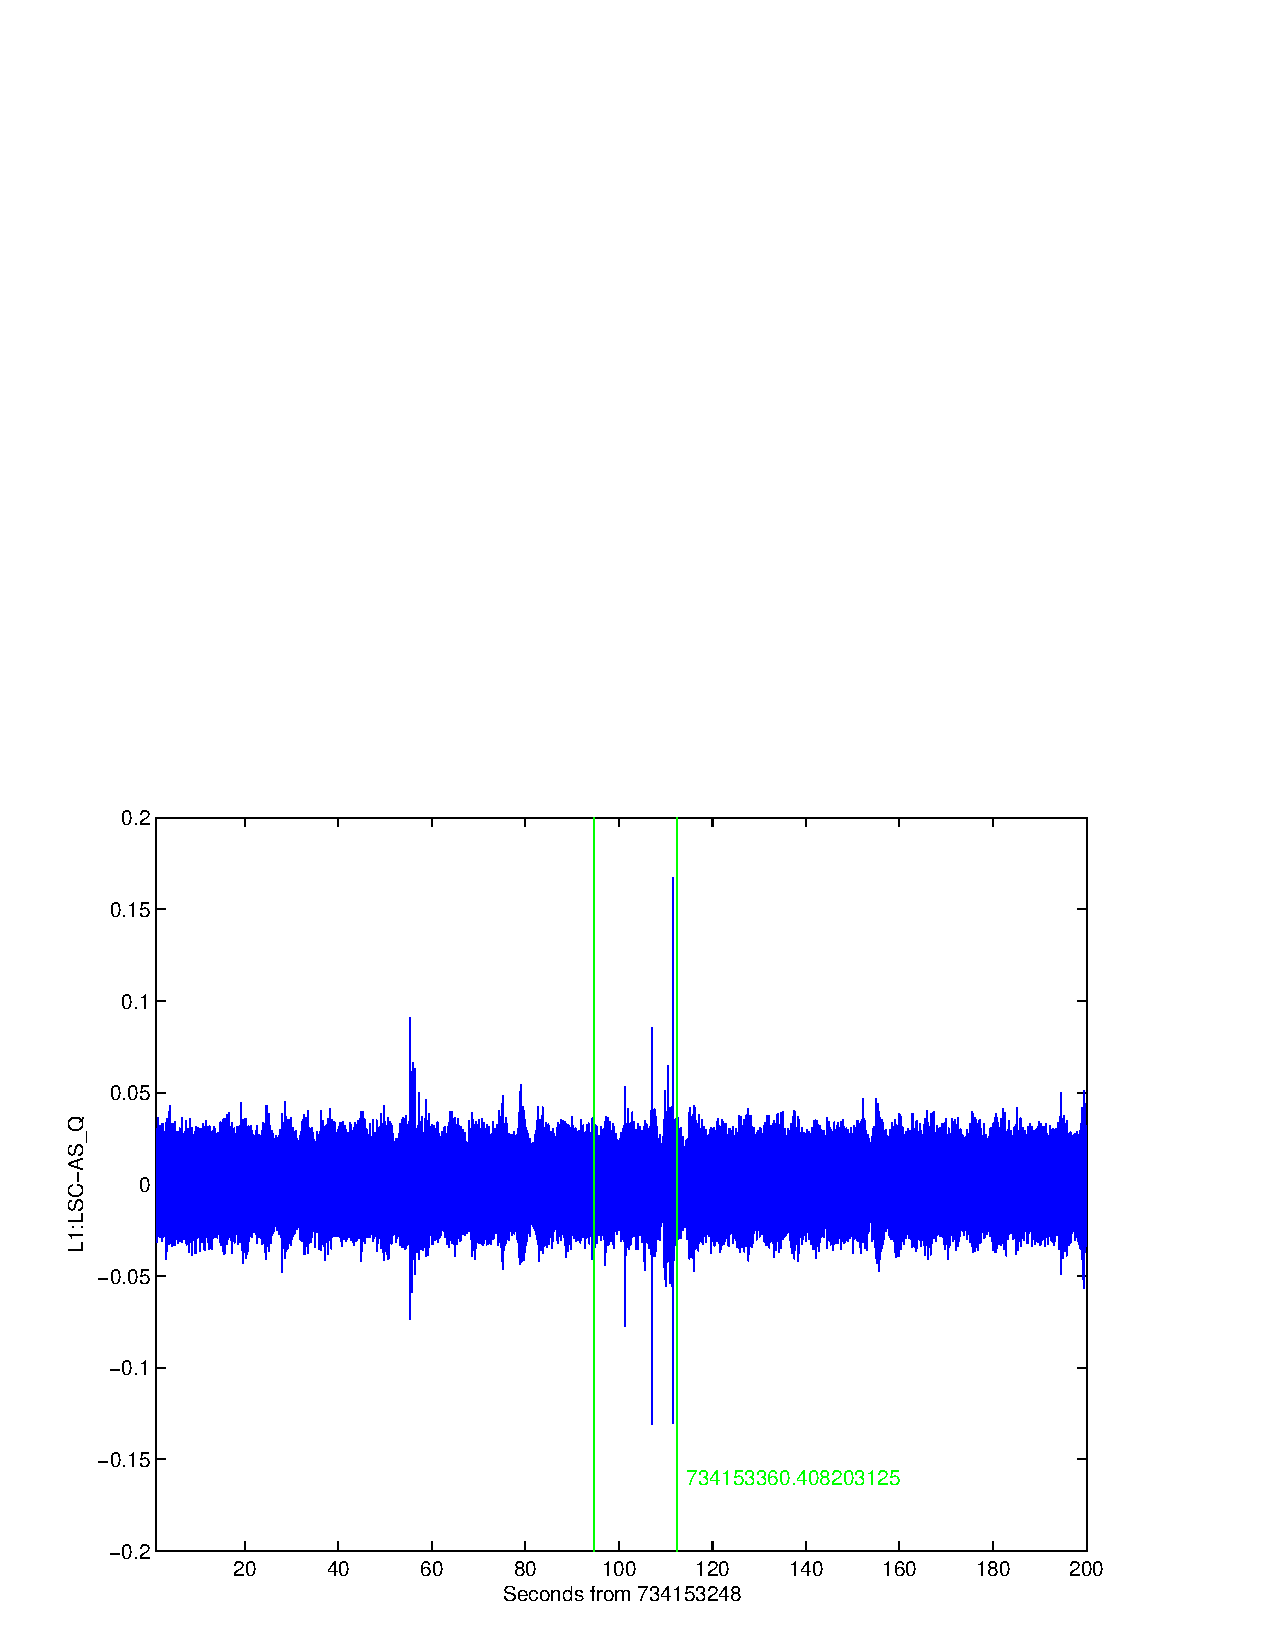
\includegraphics[width=0.475\linewidth]{figures/pipeline/trigger_734153360_as_q}\\
(iii) & (iv) \\
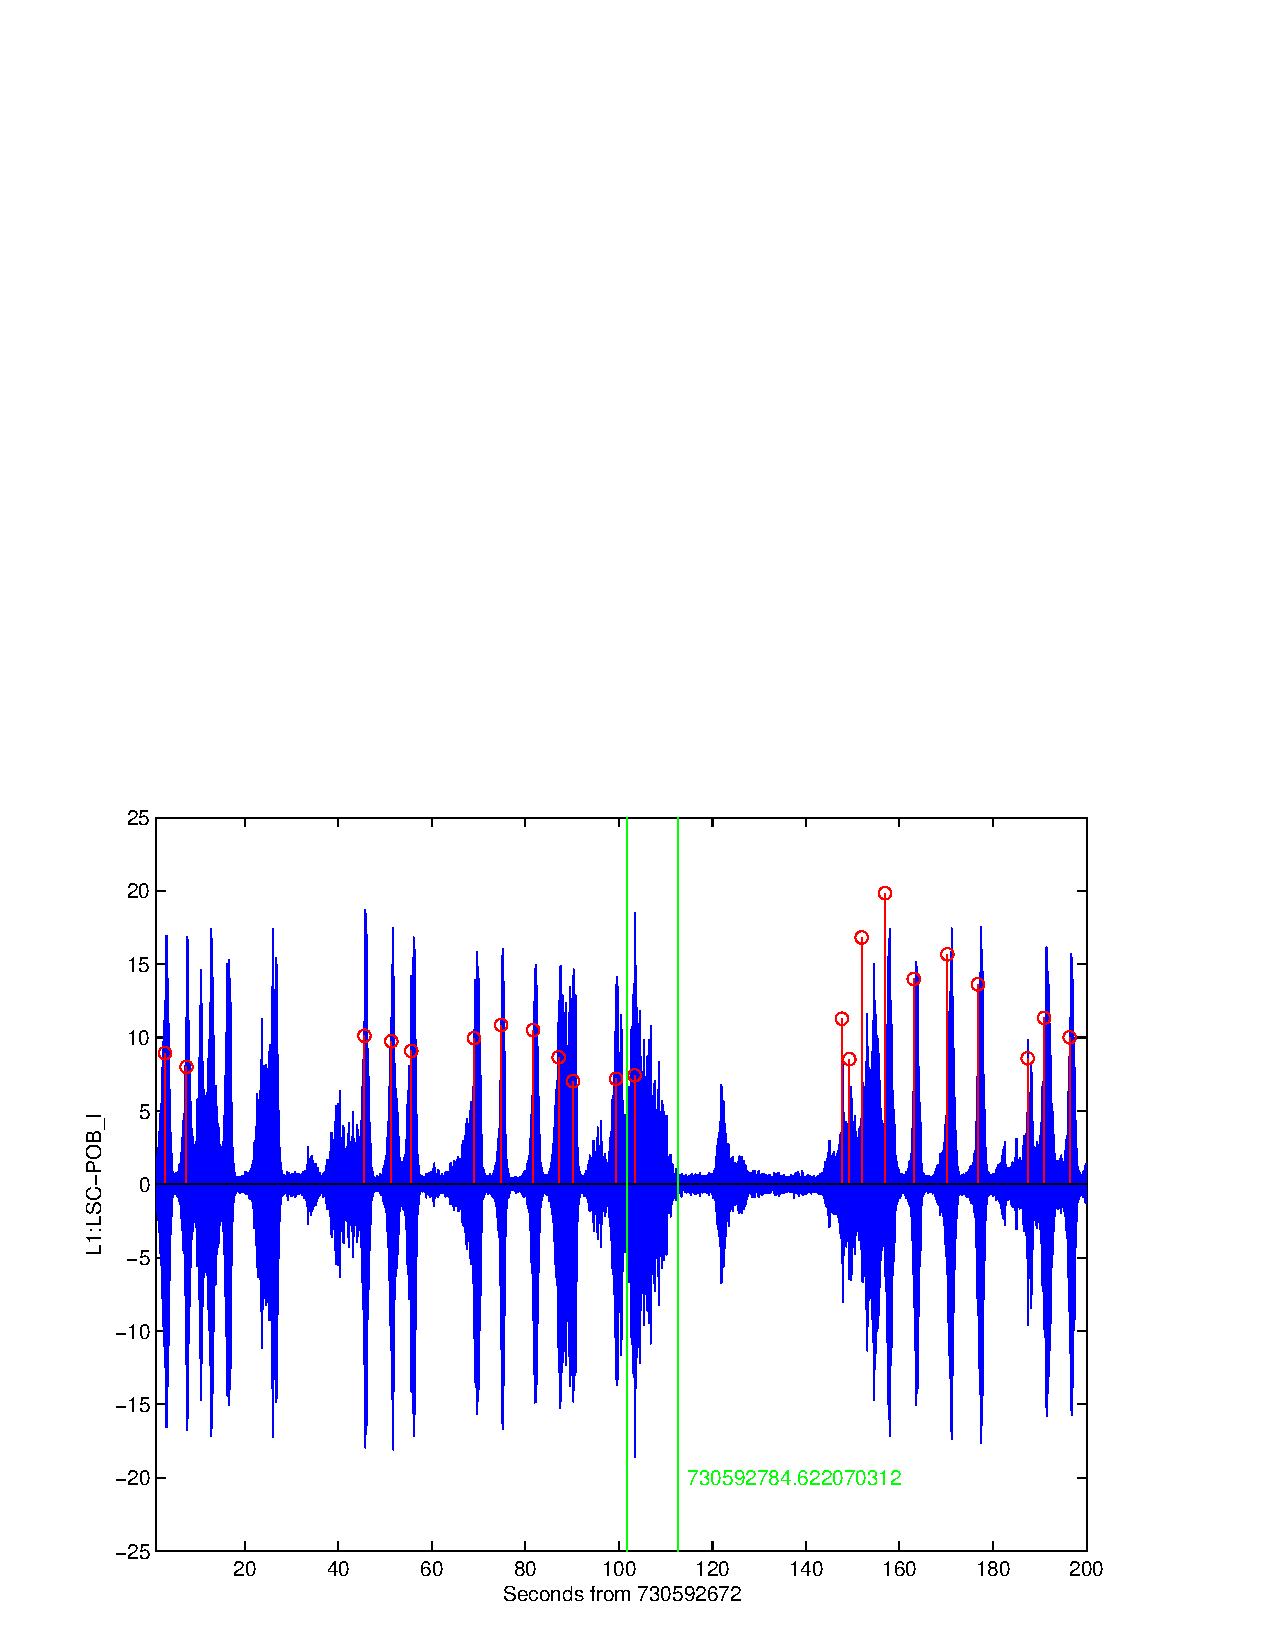
\includegraphics[width=0.475\linewidth]{figures/pipeline/trigger_730592784_pob_i} &
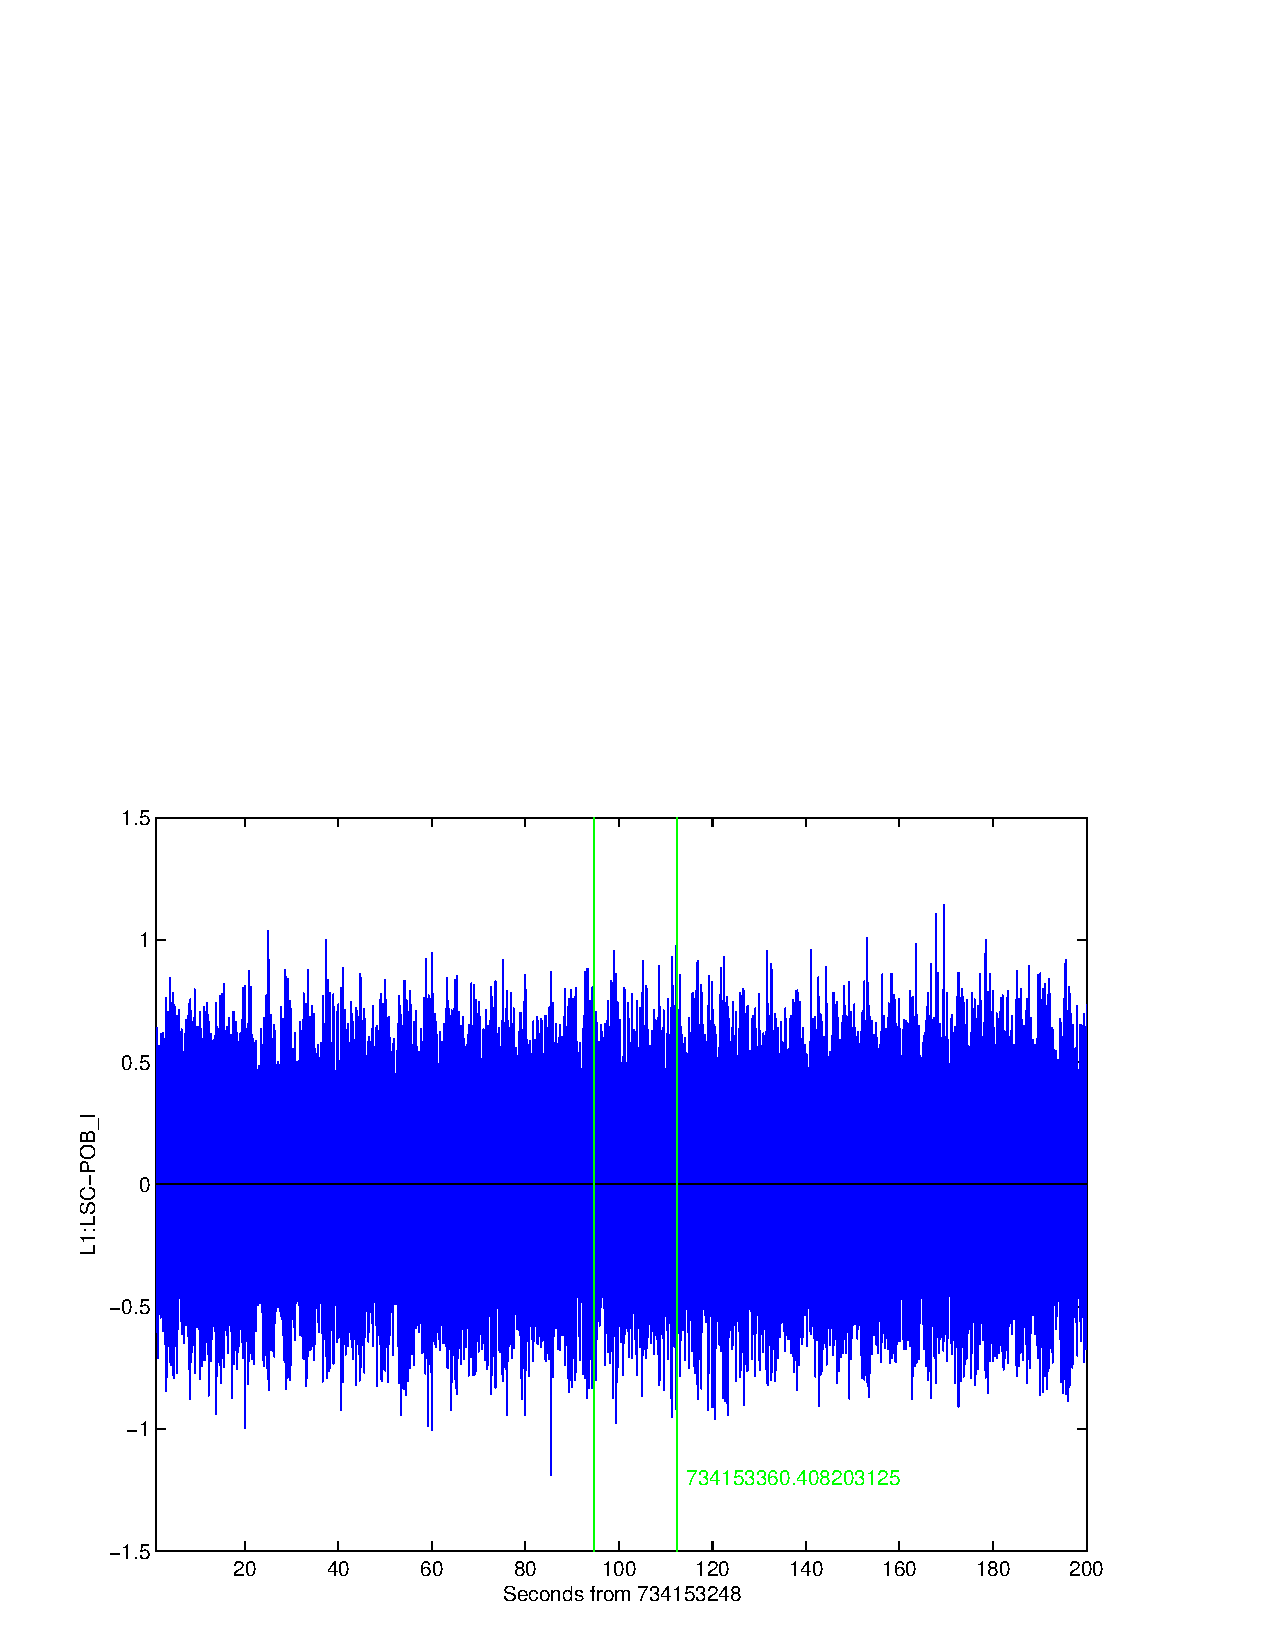
\includegraphics[width=0.475\linewidth]{figures/pipeline/trigger_734153360_pob_i}\\
\end{tabular}
\end{center}
\caption[Auxiliary Channel Veto Investigation of Two Candidate Triggers]{%
An auxiliary channel veto investigation of two candidate triggers. Panel (i)
shows the gravitational wave channel, L1:LSC-AS\_Q, high passes above 100 Hz
for a an inspiral trigger at GPS time 730592784 with a signal-to-noise ratio
$\rho = 10.6$. The vertical line shows the time of the inspiral trigger.
Panels (iii) shows the auxiliary interferometer channel L1:LSC-POB\_I high
passed above 70 Hz. The vertical lines with circles show the location of
glitchMon triggers produced by the noise in L1:LSC-POB\_I. By excluding
inspiral triggers within a time window of these glitchMon triggers, we can
reduce the number of false event candidates in the pipeline. For contrast,
panel (ii) shows an gravitational wave channel high passed above 100 Hz for
an inspiral trigger at GPS time 734153360. This trigger has a similar
signal-to-noise ratio, $\rho = 10.9$, as the trigger in panel (i). For this
trigger there does not seem to be a correlated noise source in the auxiliary
channel L1:LSC-POB\_I shown high passed above 70 Hz in panel (iv).  
}
\end{figure}


\begin{figure}[p]
\label{f:s2noisecurve}
\vspace{5pt}
\begin{center}
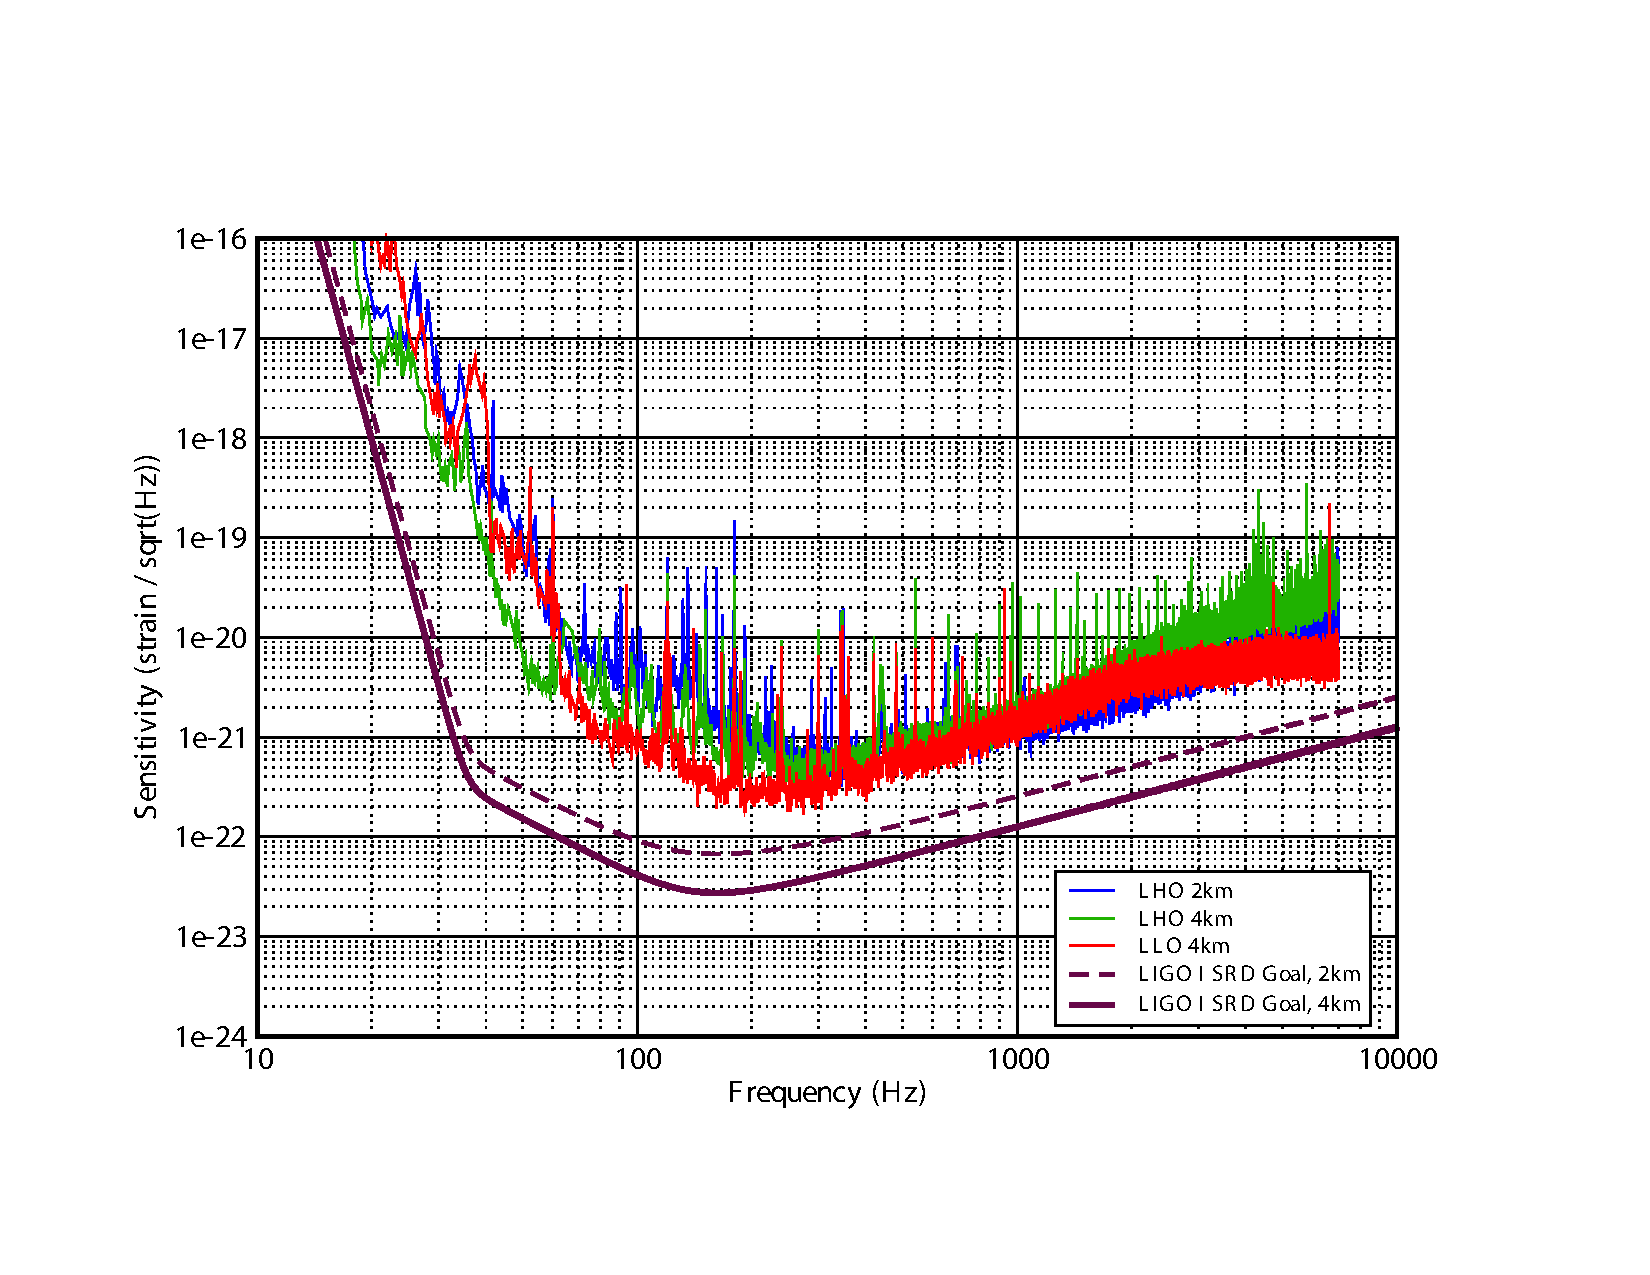
\includegraphics[width=\textwidth]{figures/pipeline/G030379-00}    
\end{center}
\caption[Sensitivity of LIGO Interferometers During S2]{%
Typical sensitivities of the three LIGO interferometers during the second LIGO
science run shown as strain amplitude spectral density,
$\tilde{h}/\sqrt{\mathrm{Hz}}$. The smooth solid curve shows the design
sensitivity (SRD Goal) of the $4$~km interferometers and the smooth dashed
curve shows the design sensitivity of the $2$~km interferometer.
}
\end{figure}

\begin{table}[p]
\label{t:s2dqresults}
\begin{center}
\begin{tabular}{lcccccccc}
H1 Data Quality Cut      &$T_\mathrm{total}$&$T_\mathrm{play}$&$T_\mathrm{done}$&$\rho>8$&$\rho>10$&$\rho>12$ \\
(1)                      &(2)     &(3)    &(4)    &(5)     &(6)     &(7)\\\hline
ASQ\_LOWBAND\_OUTLIER    &  14741 &  1990 &  1536 &   625  &  178   &   2 \\
ASQ\_OUTLIER\_CLUSTER    &  20407 &  1800 &  1800 &     0  &    0   &   0 \\
ASQ\_OUTLIER\_CORRELATED &   3126 &   558 &   456 &   390  &  167   &   2 \\
ASQ\_UPPERBAND\_OUTLIER  &  22817 &  1876 &  1876 & 15435  &10159   &7574 \\
AS\_PD\_SATURATION       &     72 &     5 &     0 &     0  &    0   &   0 \\
MICH\_FILT               & 118807 & 11400 & 11400 &  4443  & 3922   &3185 \\
\hline\hline
\\
H2 Data Quality Cut      &$T\mathrm{total}$&$T_\mathrm{play}$&$T_\mathrm{done}$&$\rho>8$&$\rho>10$&$\rho>12$ \\
(1)                      &(2)     &(3)    &(4)    &(5)     &(6)     &(7)  \\\hline
AS\_PD\_SATURATION        &    4   &   0   &   0  &    0  &    0   &   0 \\
MICH\_FILT                &64368   &6570   &5648  & 1294  &  164   &   7 \\
\hline\hline
\\
L1 Data Quality Cut      &$T\mathrm{total}$&$T_\mathrm{play}$&$T_\mathrm{done}$&$\rho>8$&$\rho>10$&$\rho>12$ \\
(1)                      &(2)     &(3)    &(4)    &(5)     &(6)     &(7)  \\\hline
ASQ\_LARGEP2P            &   2699 &   380 &     0  &    0 &    0  &    0 \\
ASQ\_OUTLIER\_CORRELATED &    840 &    60 &    60  &    0 &    0  &    0 \\
AS\_PD\_SATURATION       &    646 &    61 &    10  &  813 &  119  &    6 \\
MICH\_FILT               & 203539 & 21696 & 17794  & 6393 &  497  &   32 \\
NONSTAND\_CTRLS          &   4020 &   843 &    18  &    0 &    0  &    0 \\
\end{tabular}
\end{center}
\caption[Inspiral Triggers Generated at Times of Data Quality Cuts]{
The table shows the inspiral triggers generate from science mode data with the
mandatory data quality cuts applied. For each discretionary data quality cut
applied a given interferometer (1), the amount of time that would be excluded
from the total science mode data by the cut is given (2). Since we tune data
quality cuts on playground data, the amount of playground time excluded is
also shown (3) and the amount of playground data analyzed for triggers (4).
These may differ for reasons explained in section \ref{ss:datamanagement}. The
number inspiral triggers generated when a particular data quality cut is
active is shown for different signal-to-noise thresholds (5--7). To generate
the triggers, interferometer data was high passed above $50$~Hz in the time
domain and a low frequency cutoff of $70$~Hz was applied to frequency domain.
Template banks were generated with a minimal match of $0.97$ and the
signal-to-noise threshold for the matched filter was set to $\rho_\ast = 8$. A
$\chi^2$ veto with $8$ bins applied with a threshold of $\chi^2 < 20 (8 +
0.03^2 \rho^2)$. 
}
\end{table}

\begin{table}[p]
\label{t:s2dqchoice}
\begin{center}
\begin{tabular}{ll}
Discretionary Data Quality Cut  & Applied \\\hline\hline
MICH\_FILT                 & No \\
\multicolumn{2}{l}{\parbox{\linewidth}{\footnotesize The cut would exclude a
large number of triggers, but would reduce the amount of data in the search
significantly. It was decided not to apply this cut and to try and exclude
false triggers from these times by a combination of coincidence, vetoes and
reducing the $\chi^2$ threshold.}}\\
\\
AS\_PD\_SATURATION        & Yes \\
\multicolumn{2}{l}{\parbox{\linewidth}{\footnotesize Clear correlation with
inspiral triggers with large signal-to-noise ratios in L1 and the study
described in section \ref{ss:photodiode} suggest that this should be used. The
lack of correlated trigger in H1 was due to the fact that the playground did
not sample any times with photodiode situations.\baselineskip=14pt}}\\
\\
ASQ\_LARGEP2P             & No \\
\multicolumn{2}{l}{\parbox{\linewidth}{\footnotesize A loud inspiral signal
could trigger this cut, so it is unsafe for use.\baselineskip=14pt}} \\
\\
NONSTAND\_CTRLS           & Yes \\
\multicolumn{2}{l}{\parbox{\linewidth}{\footnotesize Advice from experimental
team advised that detections made during this time could not be
trusted.\baselineskip=14pt}} \\
\\
ASQ\_OUTLIER\_CLUSTER     & No \\
\multicolumn{2}{l}{\parbox{\linewidth}{\footnotesize Not 
well correlated with inspiral triggers. \baselineskip=14pt}} \\
\\
ASQ\_OUTLIER\_CORRELATED  & No \\
\multicolumn{2}{l}{\parbox{\linewidth}{\footnotesize Not 
well correlated with inspiral triggers.\baselineskip=14pt}} \\
\\
ASQ\_LOWBAND\_OUTLIER     & No \\
\multicolumn{2}{l}{\parbox{\linewidth}{\footnotesize Not 
well correlated with inspiral triggers.\baselineskip=14pt}} \\
\\
ASQ\_UPPERBAND\_OUTLIER   & Yes \\
\multicolumn{2}{l}{\parbox{\linewidth}{\footnotesize Times with high upper band
noise in H1 are clearly correlated with high signal-to-noise ratio triggers.
In order to prevent the cut from begin triggered by real signals we also
require that the cut is on for more that $180$ seconds. The longest inspiral
signal in the S2 analysis is $52$ seconds.\baselineskip=14pt}}\\
\end{tabular}
\end{center}
\caption[Choice of Data Quality Cuts in S2]{%
The final selection and justification of discretionary data quality cuts for
the S2 binary neutron star and binary black hole MACHO searches.}
\end{table}

\begin{figure}[p]
\label{f:pipeline}
\begin{center}
\hspace*{-0.2in}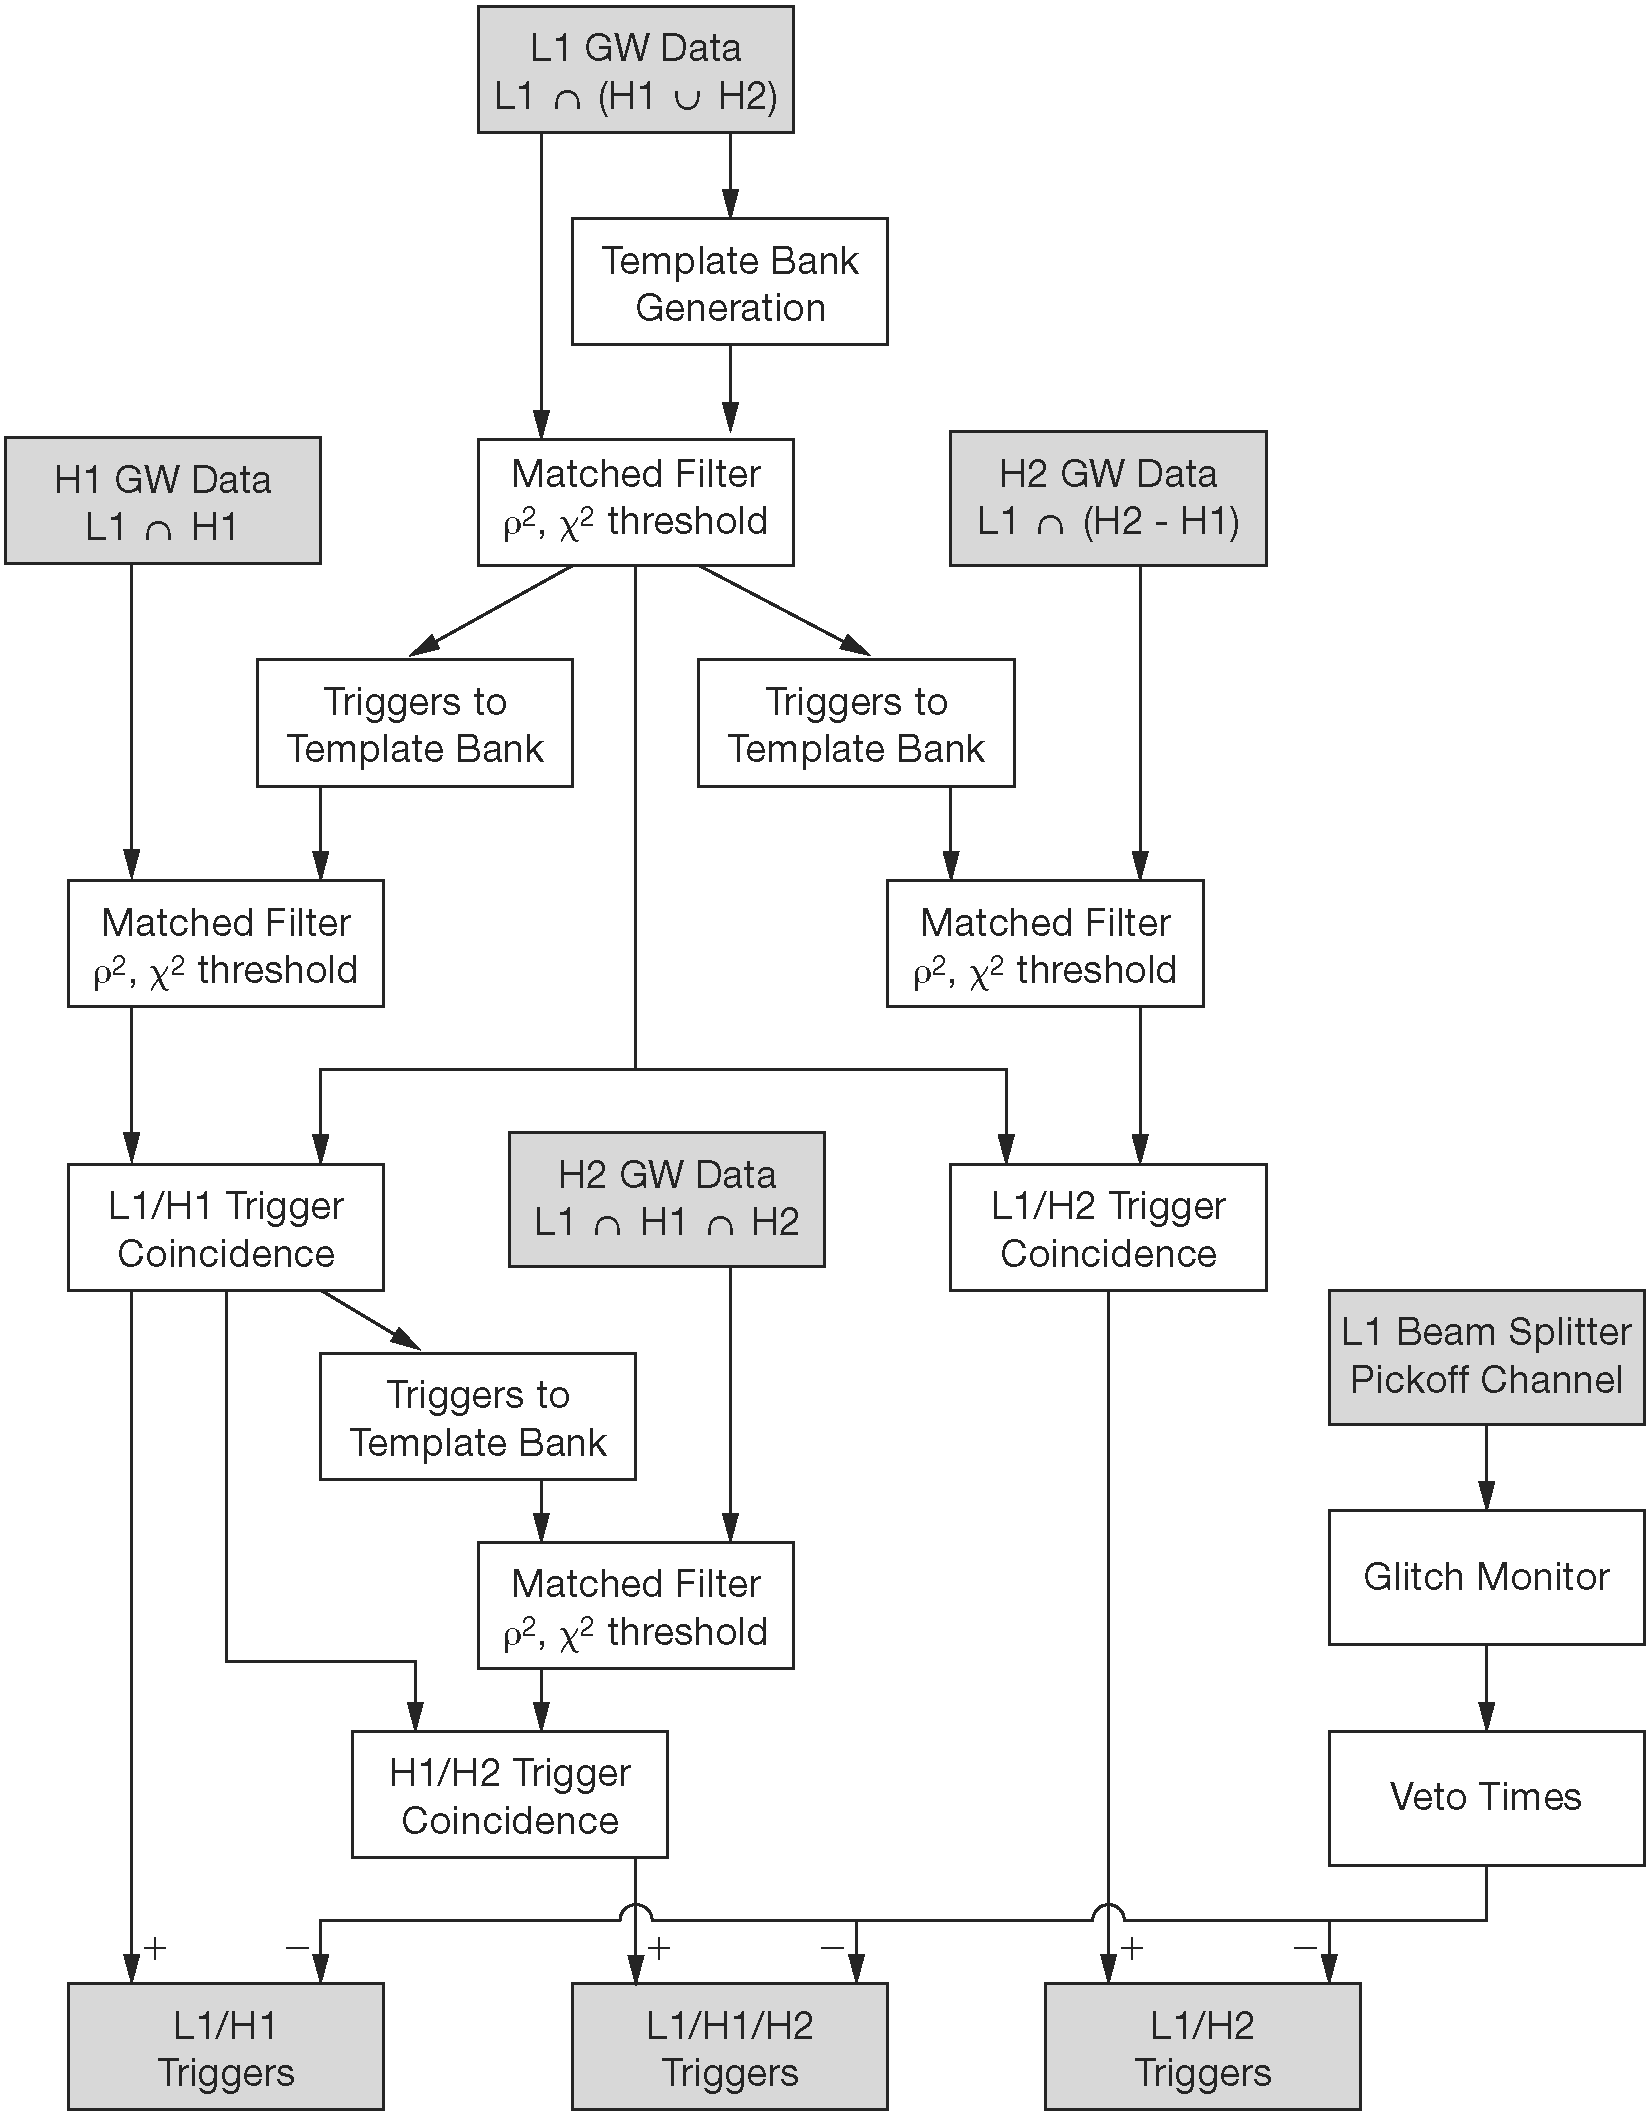
\includegraphics[width=0.6\textheight]{figures/pipeline/s2_pipeline}
\end{center}
\caption[Structure of the S2 Triggered Search Pipeline]{%
The inspiral analysis pipeline used to determine the reported upper
limit. $\mathrm{L1} \cap (\mathrm{H1} \cup \mathrm{H2})$ indicates times when
the L1 interferometer was operating in coincidence with one or both of the
Hanford interferometers. $\mathrm{L1} \cap \mathrm{H1}$ indicates times when
the L1 interferometer was operating in coincidence with the H1 interferometer.
$\mathrm{L1} \cap (\mathrm{H2} - \mathrm{H1})$ indicates times when the L1
interferometer was operating in coincidence with only the H2 interferometer.
The outputs of the search pipeline are triggers that belong to one of the
two double coincident data sets or to the triple coincident data set.}
\end{figure}

\begin{table}[p]
\label{t:fakesegslist}
\begin{center}
\begin{tabular}{llll}
Interferometer&Start&End&Duration\\
\hline
L1 &  730000000 &730010000 &  10000  \\
L1 &  731001000 &731006000 &   5000  \\
L1 &  732000000 &732003000 &   3000  \\
\hline
H1 &  730004000 &730013000 &   8000  \\
H1 &  731000000 &731002500 &   2500  \\
H1 &  732000000 &732003000 &   3000  \\
\hline
H2 &  730002500 &730008000 &   5500  \\
H2 &  731004500 &731007500 &   2500  \\
H2 &  732000000 &732003000 &   3000
\end{tabular}
\end{center}
\caption[Fake Science Segments Used to Test DAG Generation]{
The fake science segments used to construct the DAG shown in figure
\ref{f:fake_segs_dag}.
}
\end{table}

\begin{sidewaysfigure}[p]
\label{f:fake_segs_dag}
\begin{center}
\hspace*{-0.2in}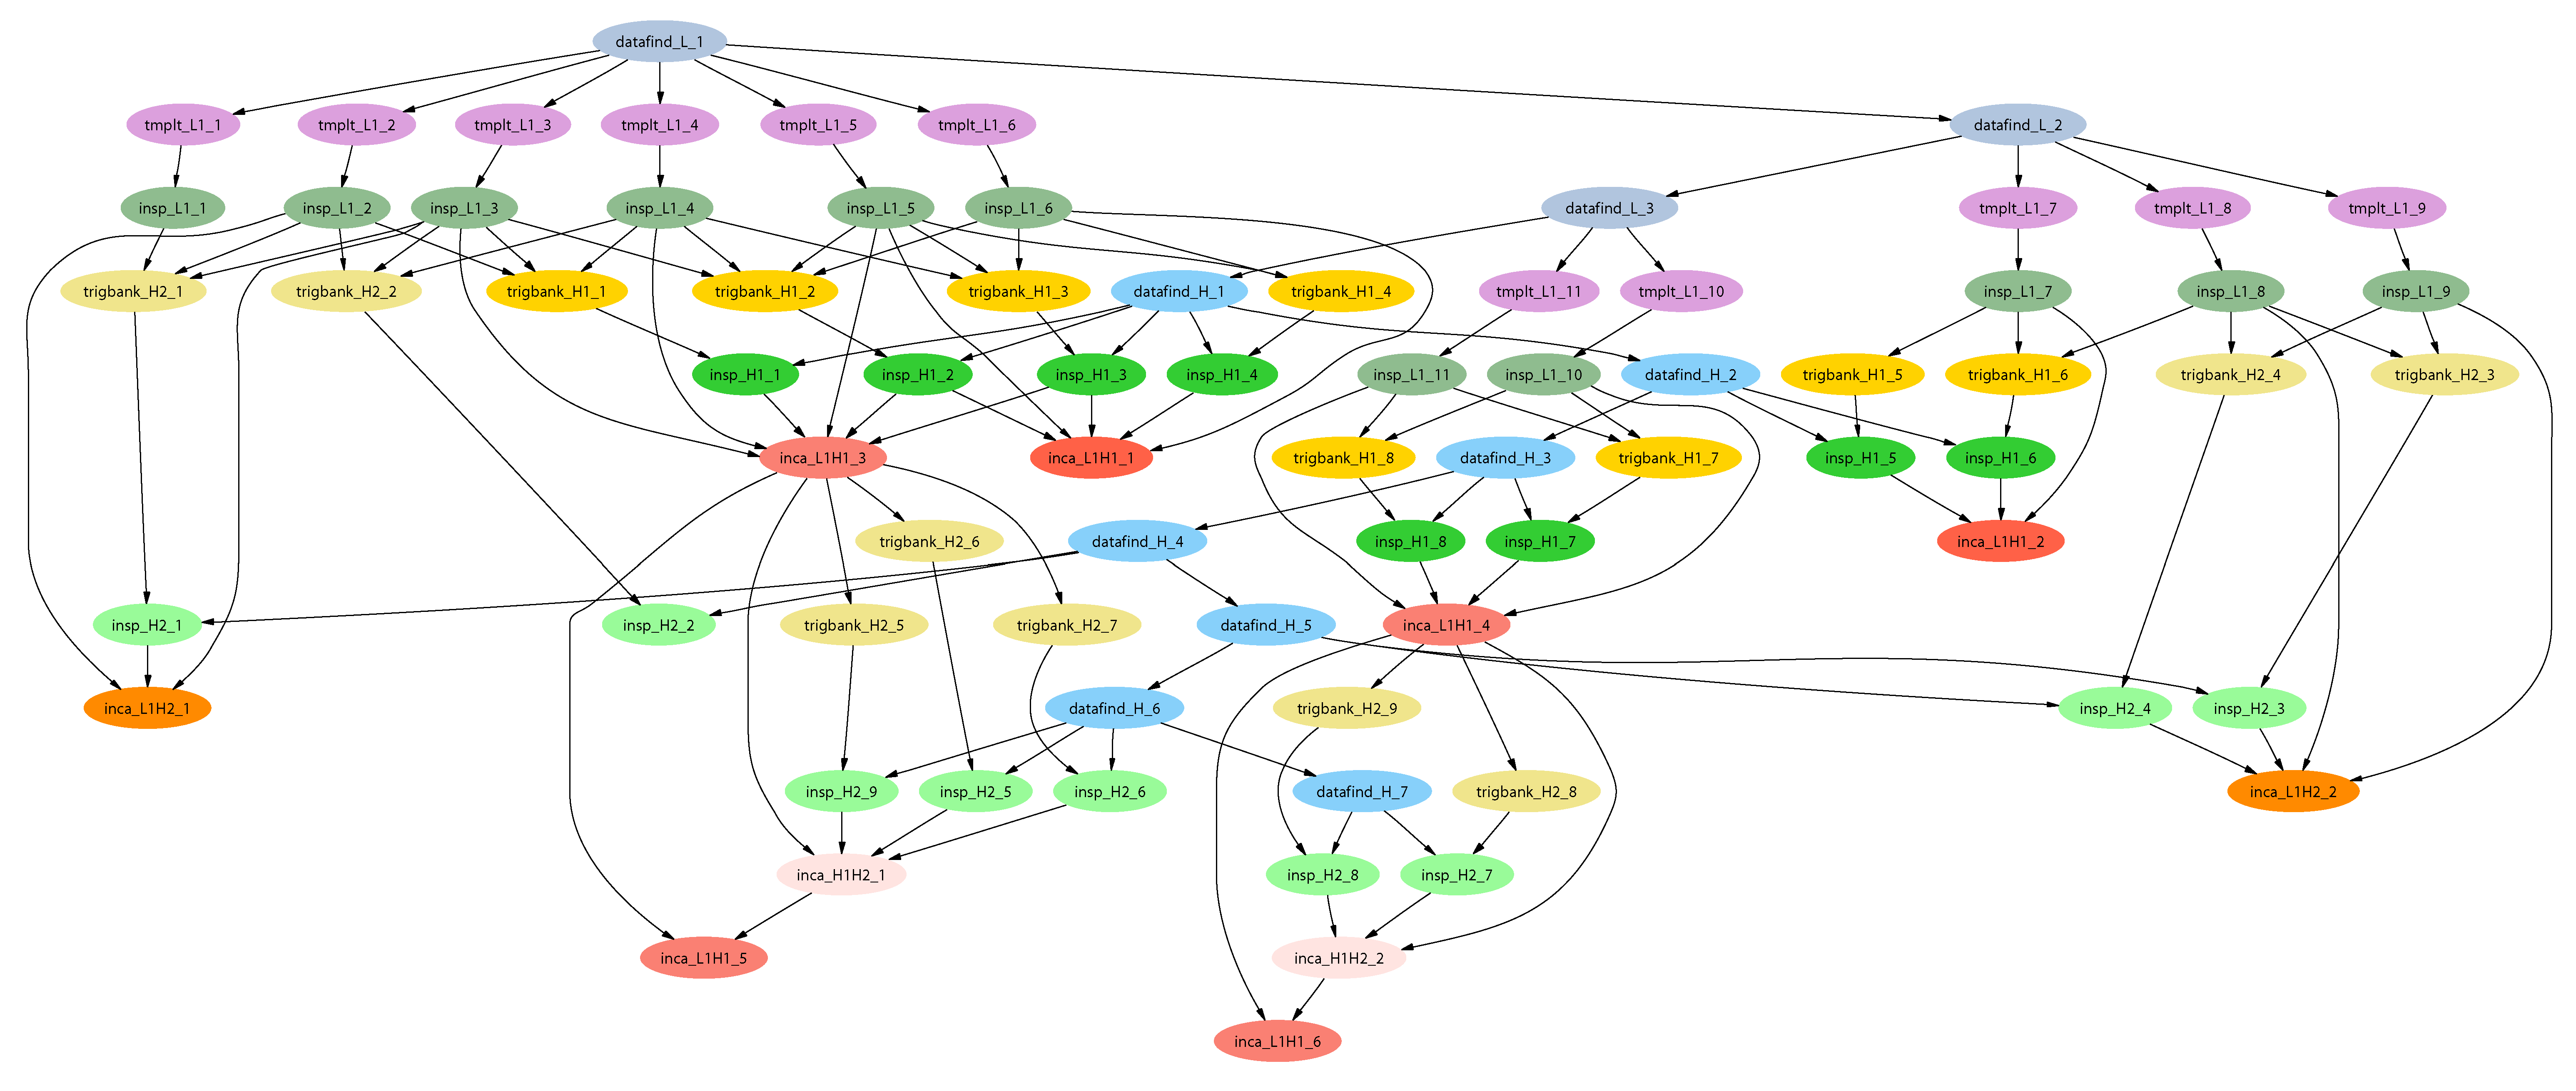
\includegraphics[width=\linewidth]{figures/pipeline/fake_segs_dag}
\end{center}
\caption[DAG Generated from Fake Segments]{%
The DAG generated from the pipeline shown in figure \ref{f:pipeline} and the
fake science segment list described in section \ref{ss:dag}. The figure shows
the structure of the DAG with all job dependencies needed to execute the S2
pipeline. Note that it appears that there are several LHO master chunks
analyzed that do not need to be filtered for a zero time lag.  These are added
to the DAG to ensure that all the data necessary for a background estimation
with a maximum time side of 500 seconds is analyzed.
}
\end{sidewaysfigure}

